\section{結果}
本節では本研究で行った2つの実験の結果について述べる.

\subsection{歌詞の印象評価}
歌詞の印象評価結果について述べる.喜怒哀楽の4クラスごとに詳説する.
\subsubsection{喜クラス}
喜の印象クラスにクラスタリングされた歌詞の評価結果について述べる.
第1グループから選出した「光の誓いが聴こえた日」,第2グループから選出した「冬三昧にはまだ遠い」,第3グループから選出した「積木遊び」の印象評価結果は以下の図4.1,4.2,4.3である.
\newpage
\begin{figure}[H]
    \centering
    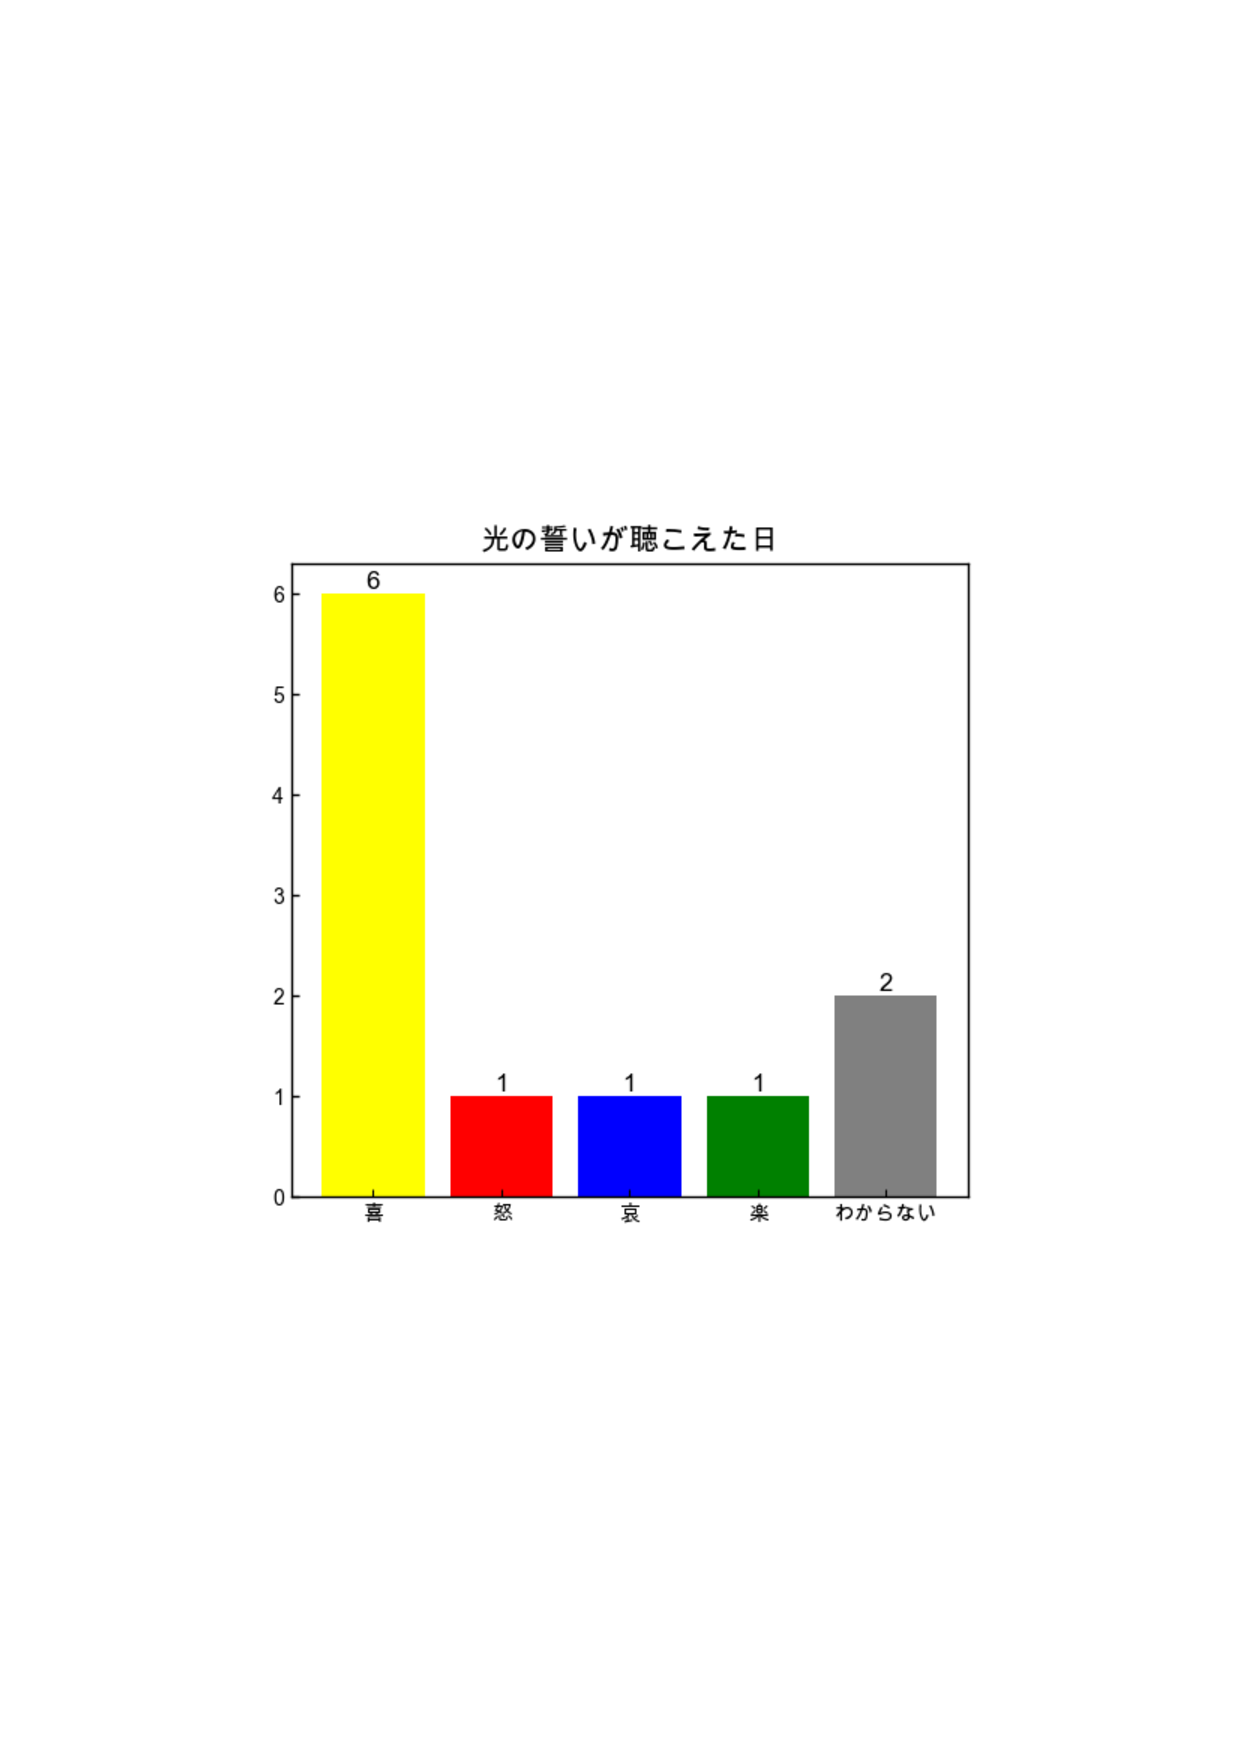
\includegraphics[width=14cm]{4313.pdf}
    \vspace{-1mm}
    \caption{歌詞 A+V+平面 第1グループ}
    \label{fig:mms}
    \vspace{5mm}
\end{figure}
第1グループから選出した「光の誓いが聴こえた日」の歌詞から実験参加者6名が喜のクラスに感じたと回答した.
怒,哀,楽のクラスを感じたと回答した人数はそれぞれ1名づつであり,わからないと回答した人数は2名であった.
実験参加者の半分以上が推定した印象を感じたことから推定結果は妥当であるといえる.
\newpage
\begin{figure}[H]
    \centering
    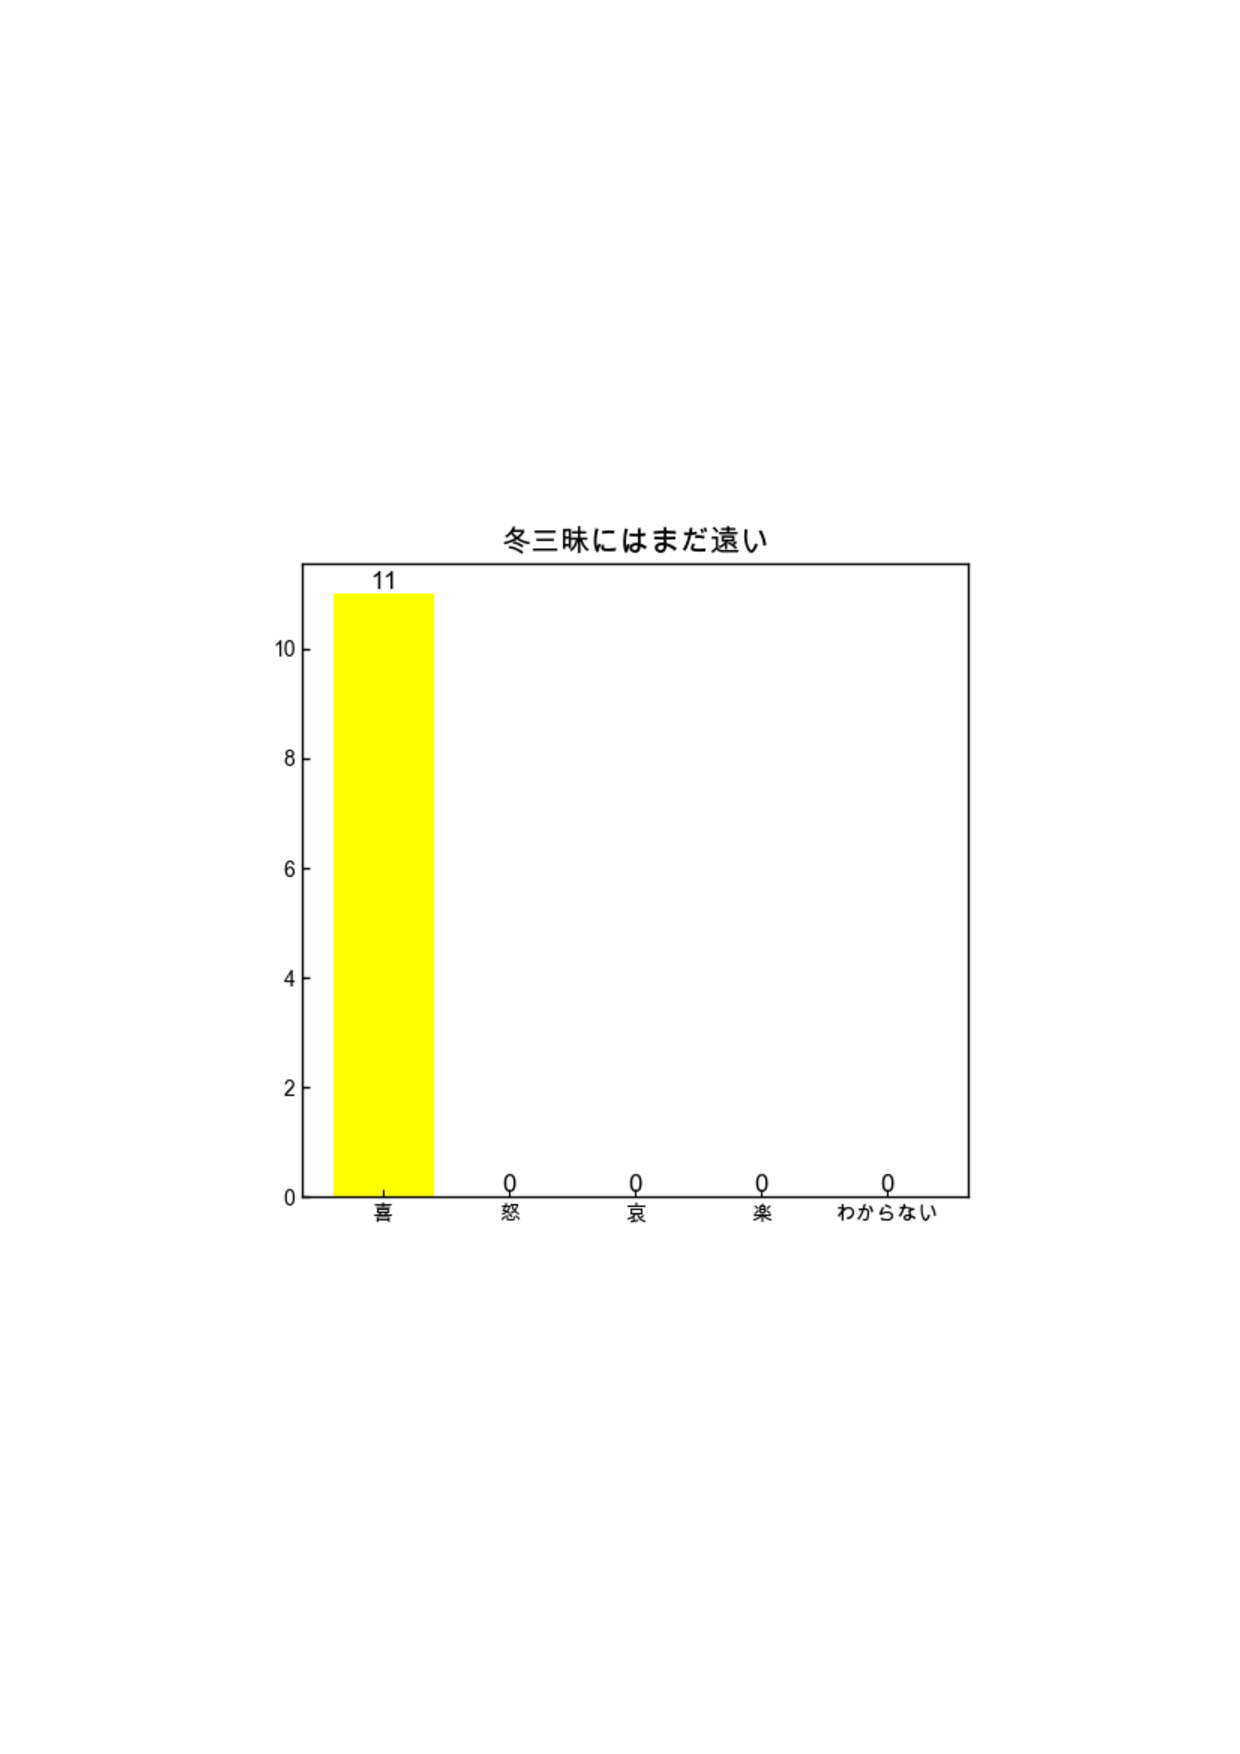
\includegraphics[width=14cm]{4314.pdf}
    \vspace{-1mm}
    \caption{歌詞 A+V+平面 第2グループ}
    \label{fig:mms}
    \vspace{5mm}
\end{figure}
第2グループから選出した「冬三昧にはまだ遠い」の歌詞から実験参加者11名全員が喜のクラスに感じたと回答した.
したがって推定結果は妥当であるといえる.
\newpage
\begin{figure}[H]
    \centering
    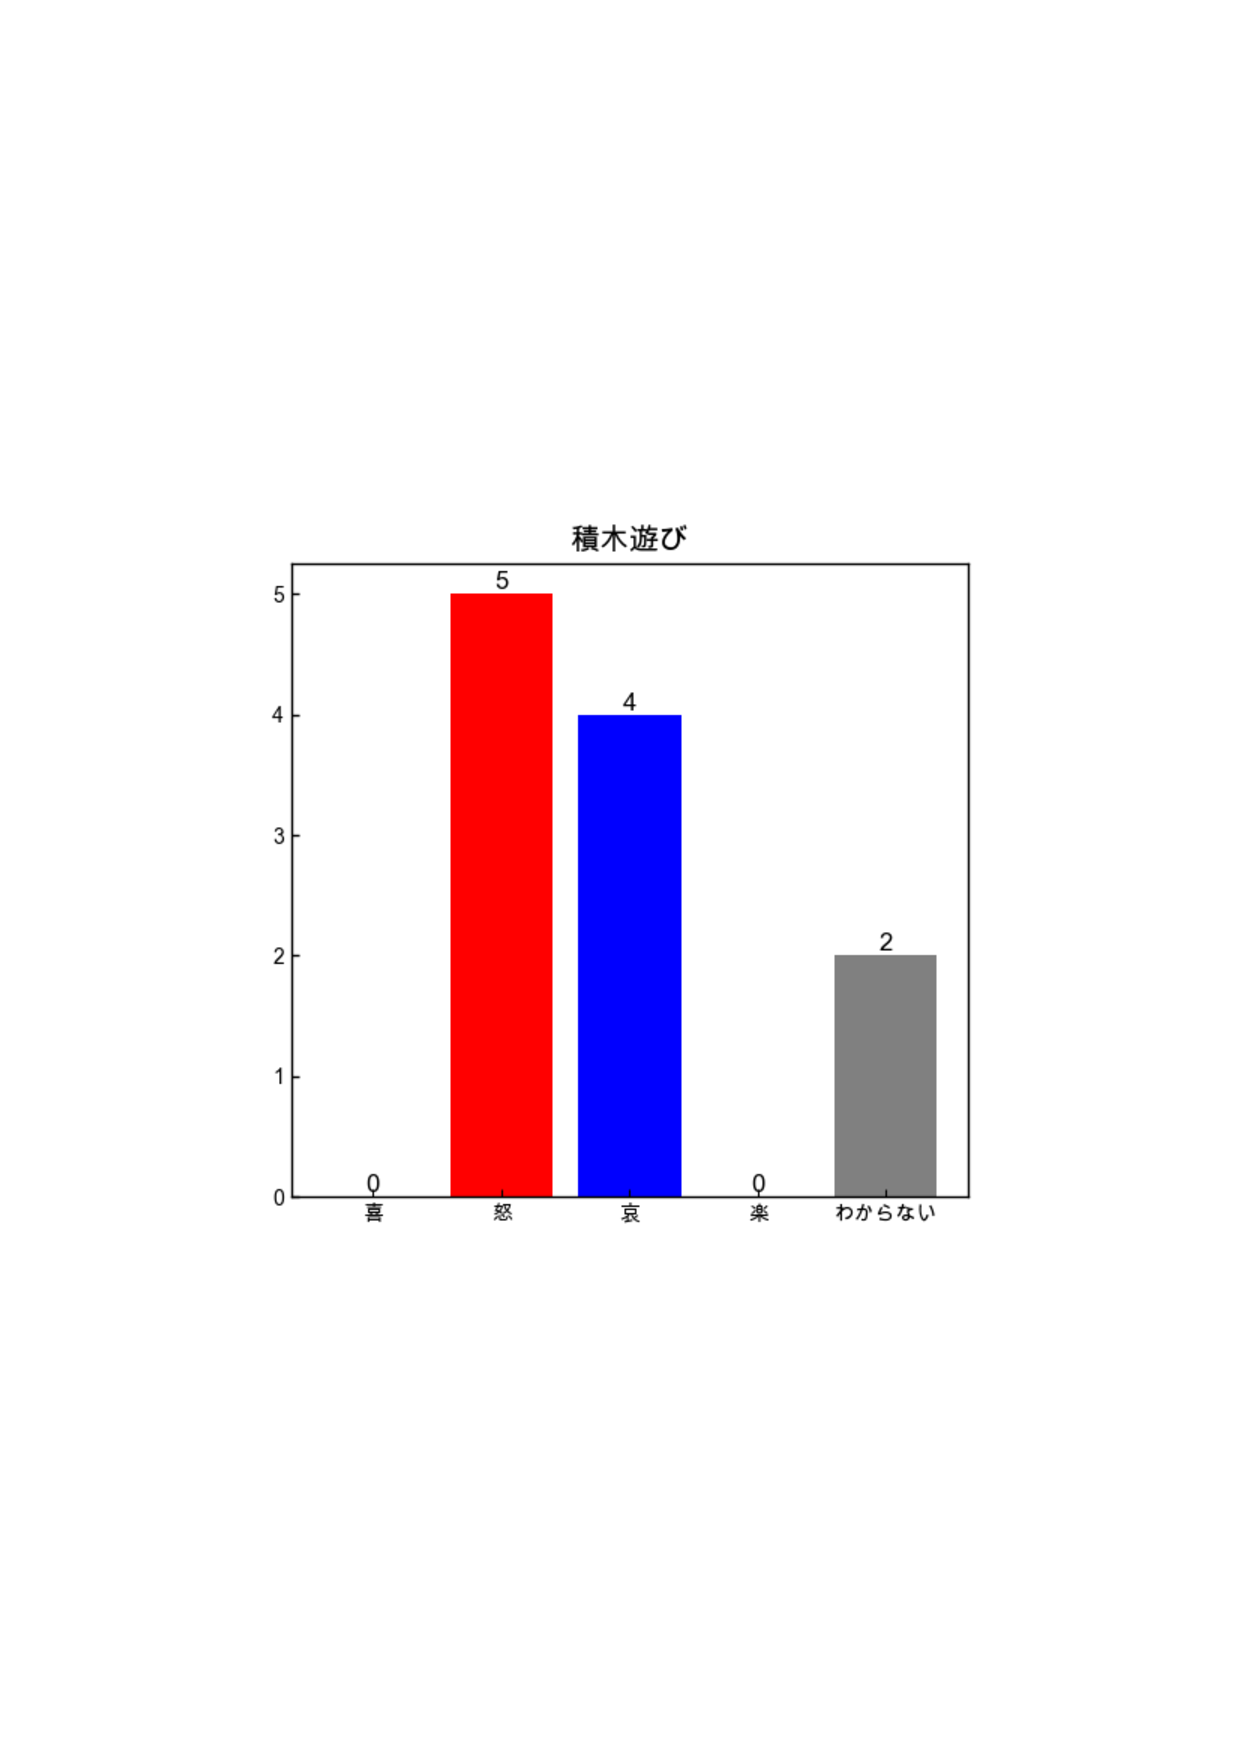
\includegraphics[width=14cm]{4315.pdf}
    \vspace{-1mm}
    \caption{歌詞 A+V+平面 第3グループ}
    \label{fig:mms}
    \vspace{5mm}
\end{figure}
第3グループから選出した「積木遊び」の歌詞から実験参加者0名が喜のクラスに感じたと回答した.
怒のクラスを感じたと回答した人数は5名,哀のクラスを感じたと回答した人数は4名,楽のクラスと感じたと回答した人はおらず,わからないと回答した人数は2名であった.
実験参加者が推定した印象を感じ取れなかったことから推定結果は不当であるといえる.
\newpage
\subsubsection{怒クラス}
怒の印象クラスにクラスタリングされた歌詞の評価結果について述べる.
第1グループから選出した「TEENAGE RIOT」,第2グループから選出した「透明人間18号」,第3グループから選出した「Da La Da Da」の印象評価結果は以下の図4.4,4.5,4.6である.
\begin{figure}[H]
    \centering
    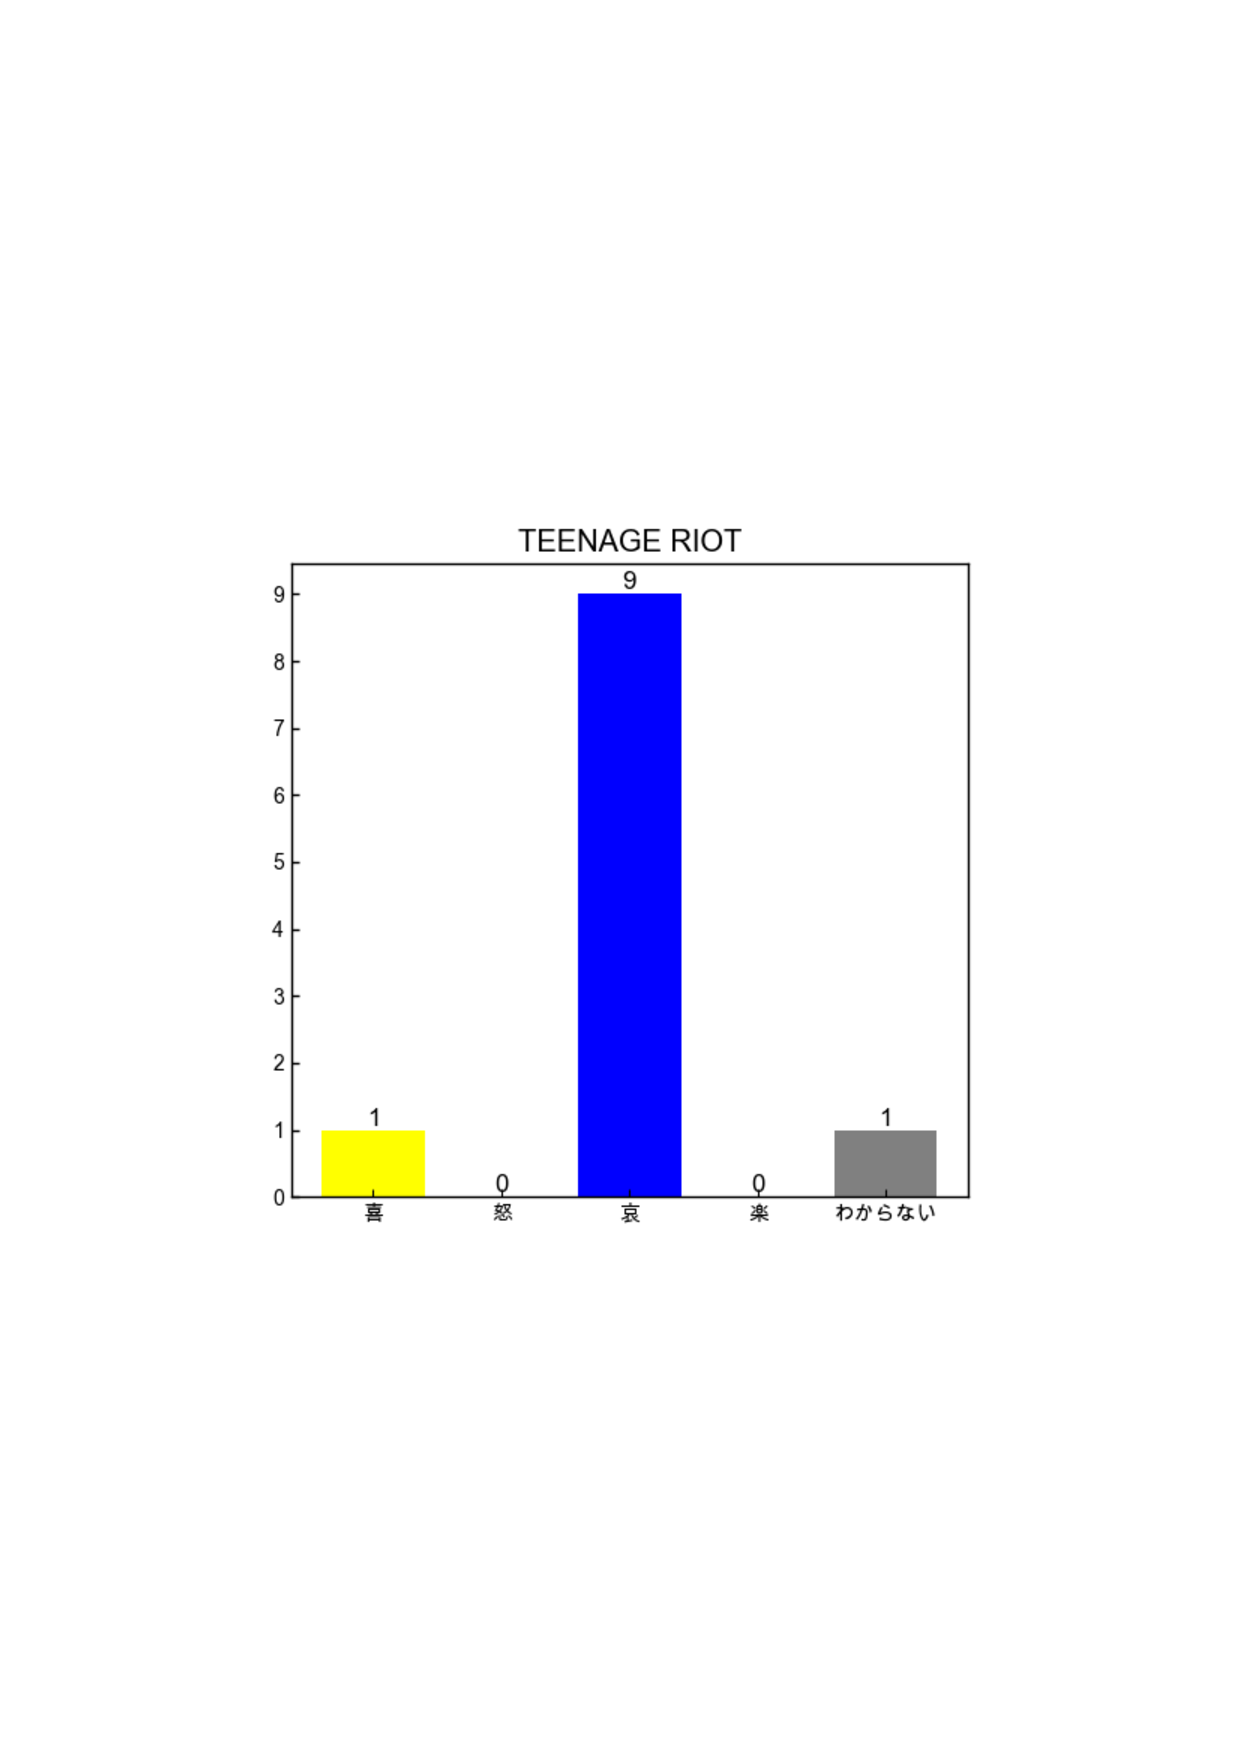
\includegraphics[width=14cm]{4316.pdf}
    \vspace{-1mm}
    \caption{歌詞 A+V-平面 第1グループ}
    \label{fig:mms}
    \vspace{5mm}
\end{figure}
第1グループから選出した「TEENAGE RIOT」の歌詞から実験参加者0名が怒のクラスに感じたと回答した.
喜のクラスを感じたと回答した人数は1名,哀のクラスを感じたと回答した人数は9名,楽のクラスと感じたと回答した人はおらず,わからないと回答した人数は1名であった.
実験参加者が推定した印象を感じ取れなかったことから推定結果は不当であるといえる.
\newpage
\begin{figure}[H]
    \centering
    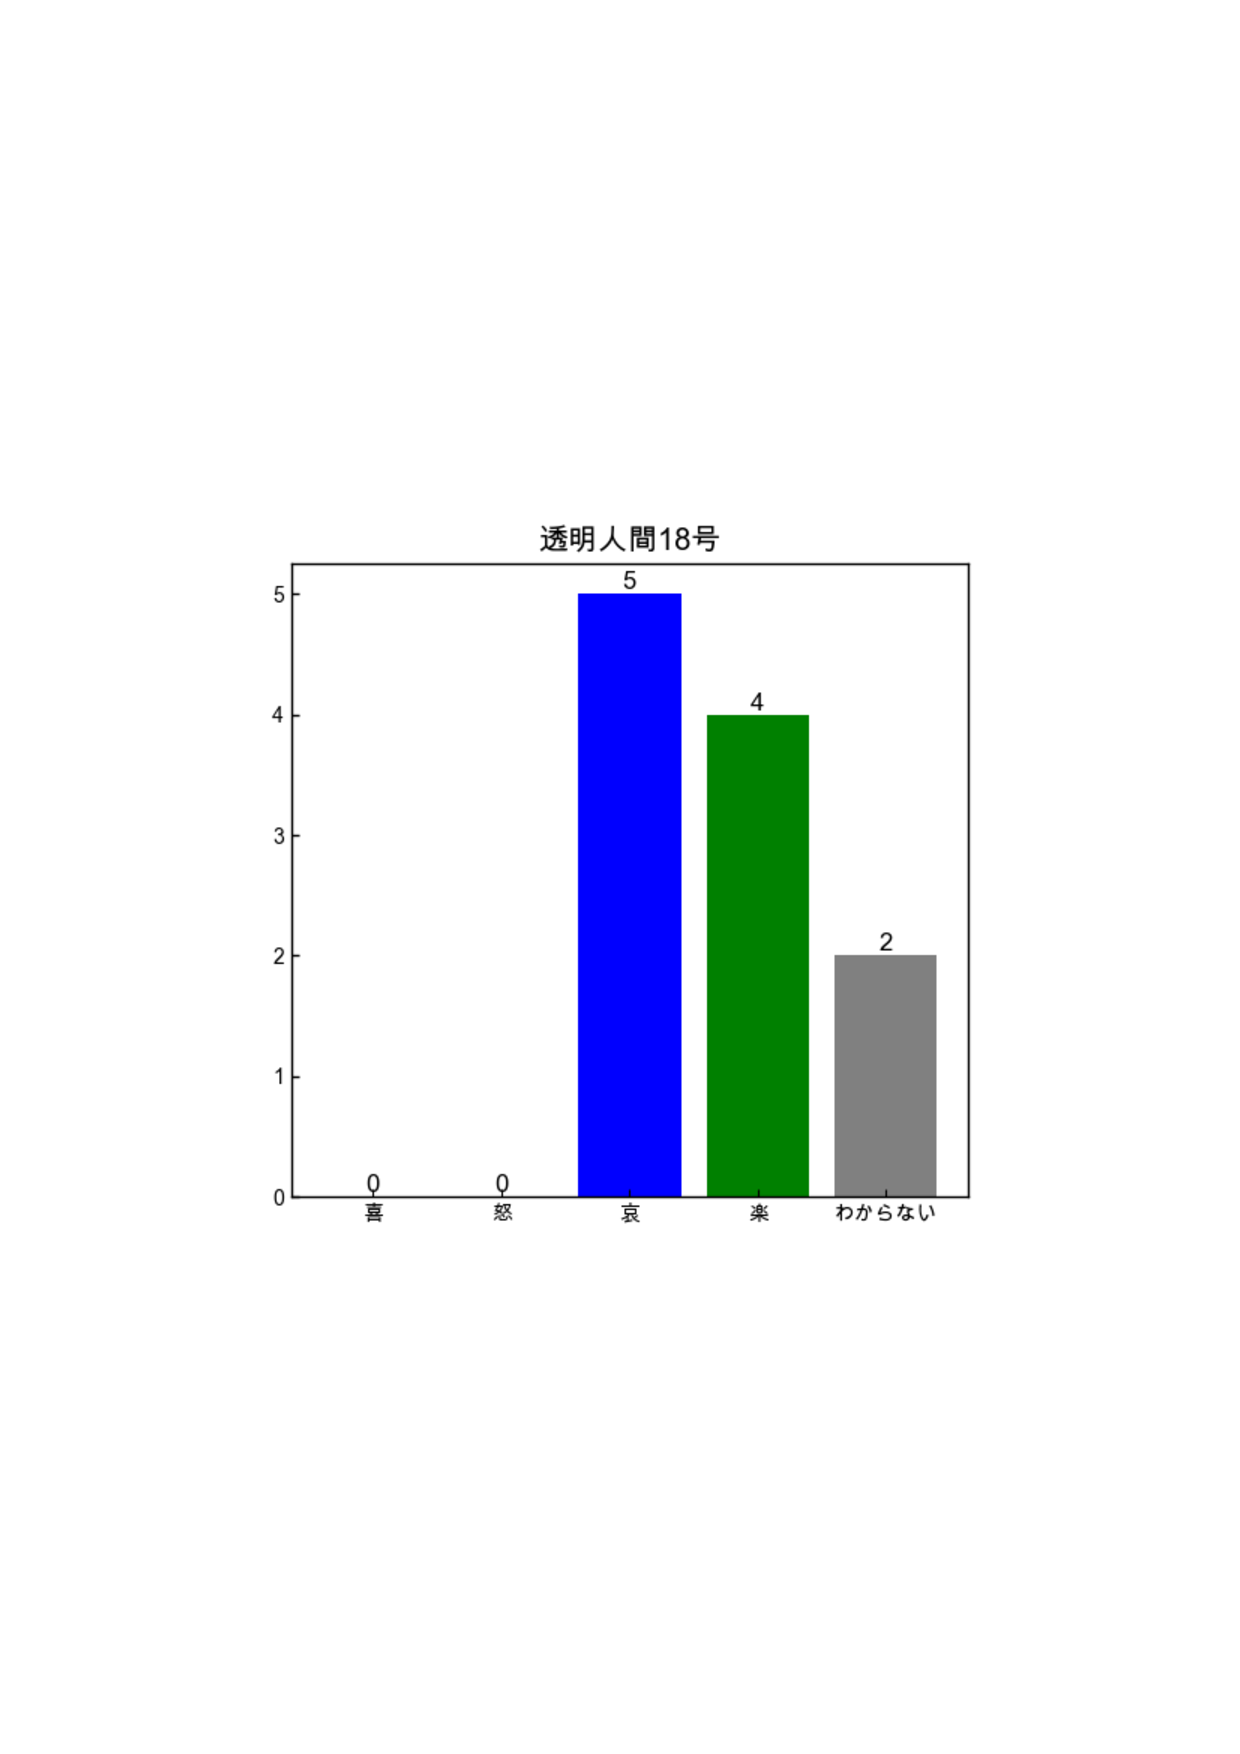
\includegraphics[width=14cm]{4317.pdf}
    \vspace{-1mm}
    \caption{歌詞 A+V-平面 第2グループ}
    \label{fig:mms}
    \vspace{5mm}
\end{figure}
第2グループから選出した「透明人間18号」の歌詞から実験参加者0名が怒のクラスに感じたと回答した.
喜のクラスを感じたと回答した人はおらず,哀のクラスを感じたと回答した人数は5名,楽のクラスを感じたと回答した人数は4名,わからないと回答した人数は2名であった.
実験参加者が推定した印象を感じ取れなかったことから推定結果は不当であるといえる.
\newpage
\begin{figure}[H]
    \centering
    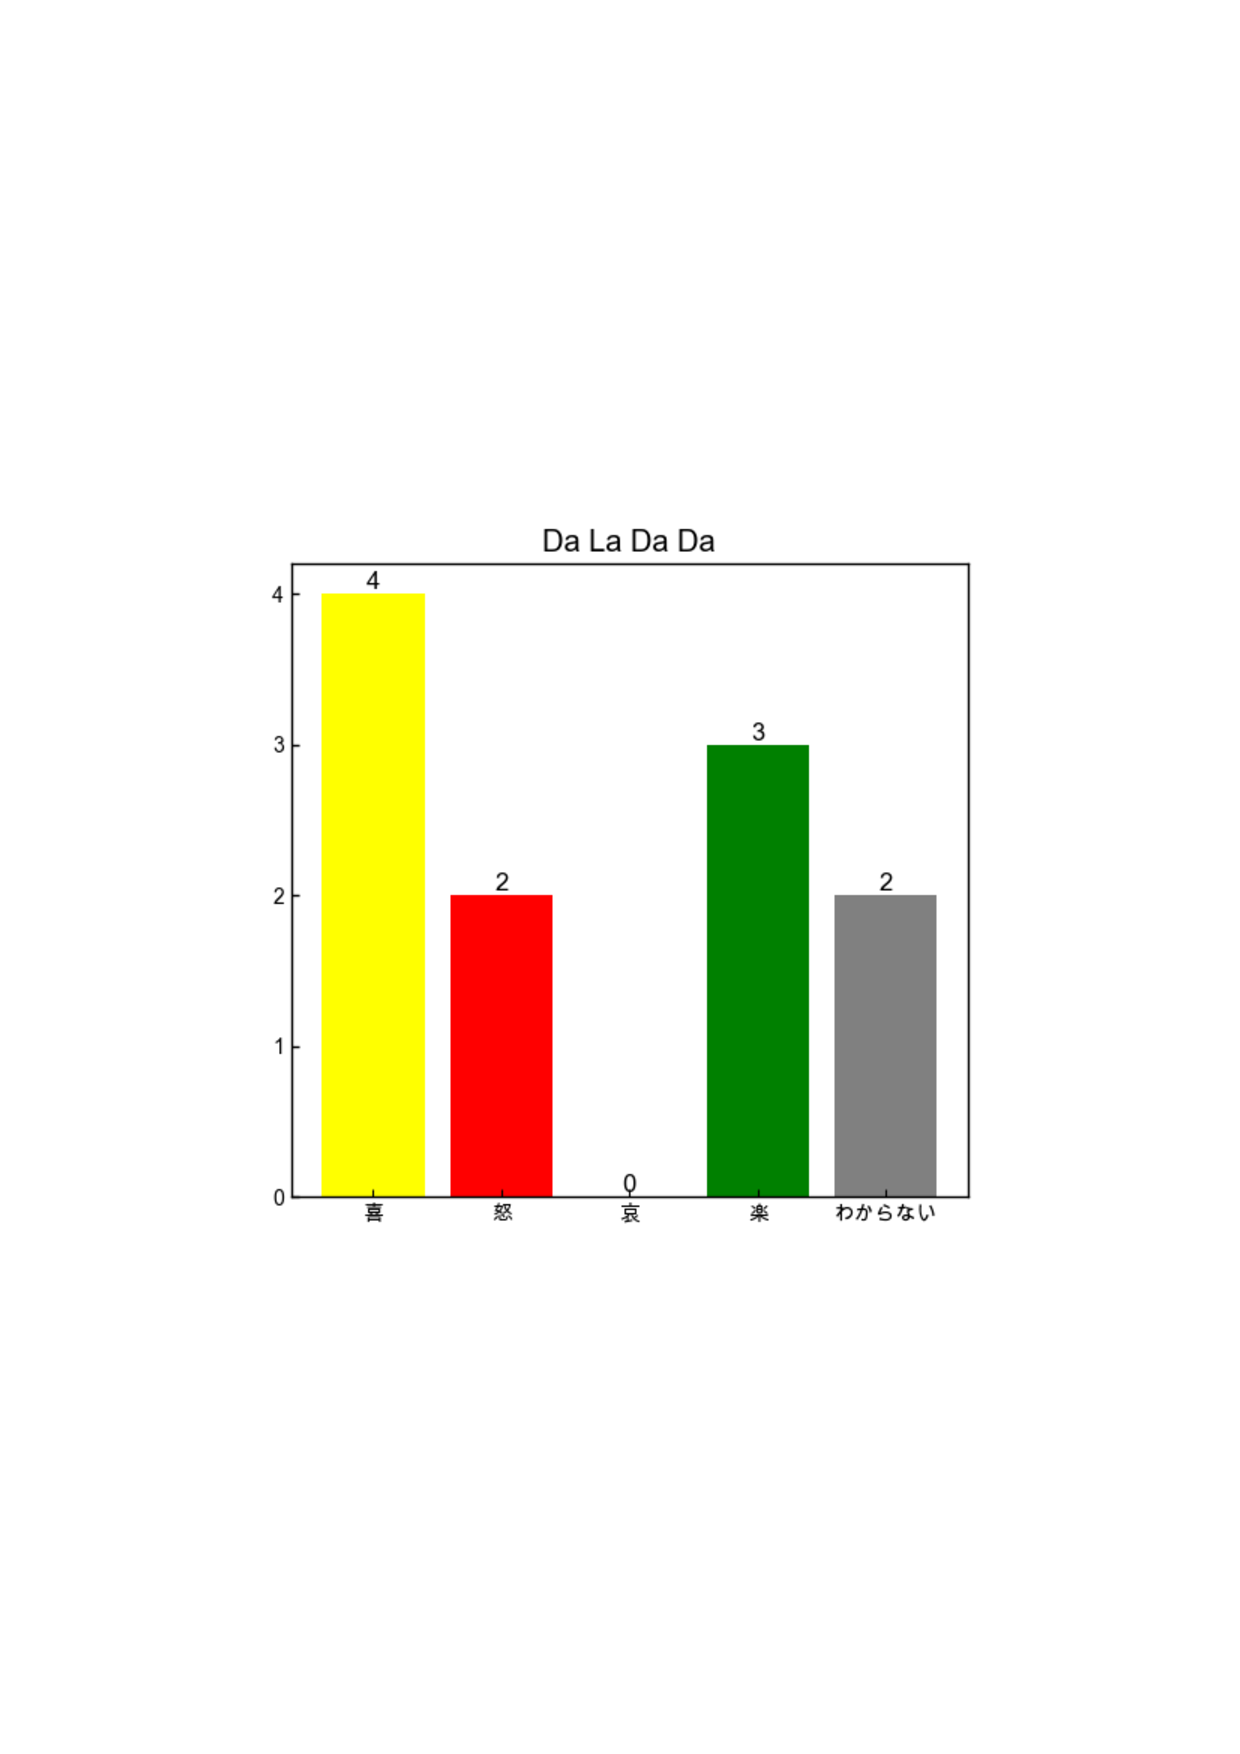
\includegraphics[width=14cm]{4318.pdf}
    \vspace{-1mm}
    \caption{歌詞 A+V-平面 第3グループ}
    \label{fig:mms}
    \vspace{5mm}
\end{figure}
第3グループから選出した「Da La Da Da」の歌詞から実験参加者2名が怒のクラスに感じたと回答した.
喜のクラスを感じたと回答した人数は4名,哀のクラスを感じたと回答した人はおらず,楽のクラスを感じたと回答した人数は3名,わからないと回答した人数は2名であった.
実験参加者の多くが推定した印象を感じ取れなかったことから推定結果は不当であるといえる.
\newpage
\subsubsection{哀クラス}
哀の印象クラスにクラスタリングされた歌詞の評価結果について述べる.
第1グループから選出した「Just be you」,第2グループから選出した「コイン」,第3グループから選出した「分別奮闘記」の印象評価結果は以下の図4.7,4.8,4.9である.
\begin{figure}[H]
    \centering
    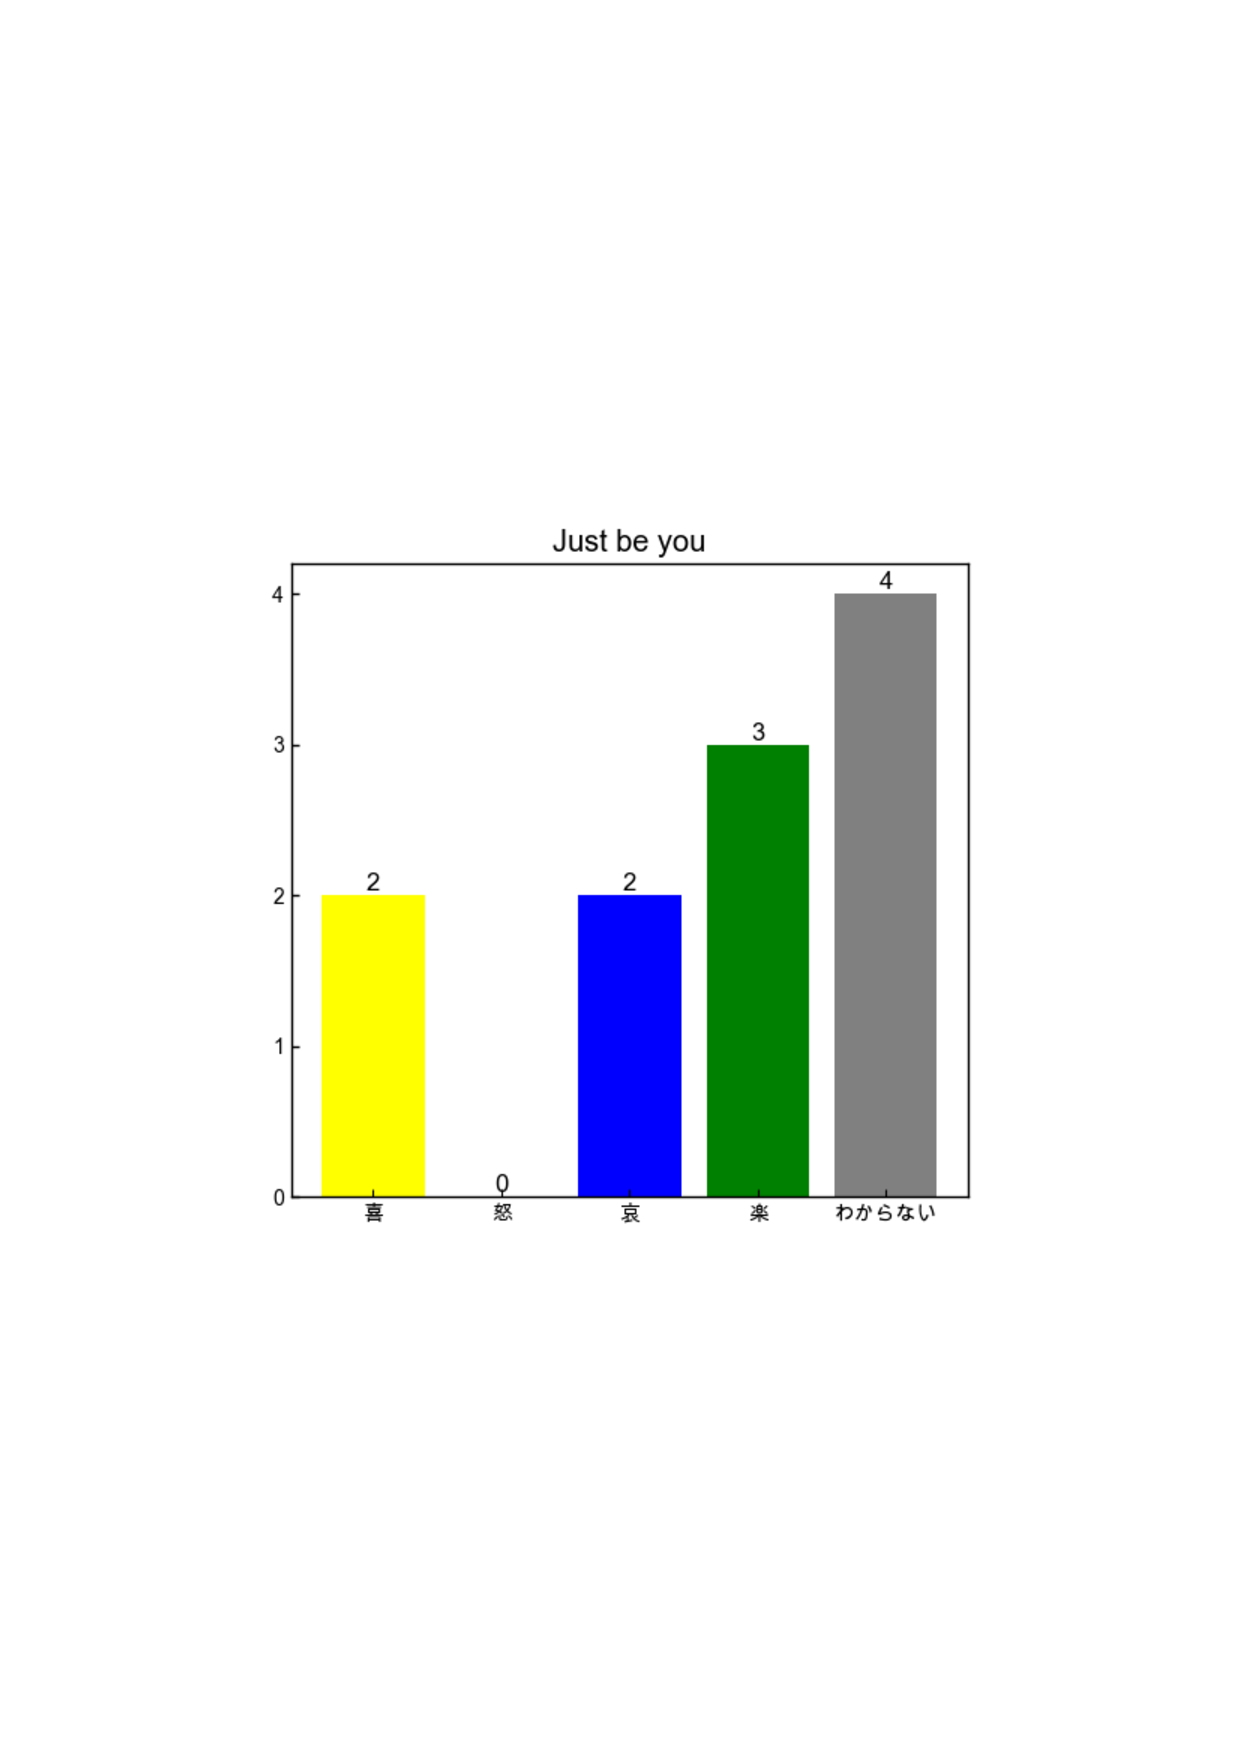
\includegraphics[width=14cm]{4319.pdf}
    \vspace{-1mm}
    \caption{歌詞 A-V-平面 第1グループ}
    \label{fig:mms}
    \vspace{5mm}
\end{figure}
第1グループから選出した「Just be you」の歌詞から実験参加者2名が哀のクラスに感じたと回答した.
喜のクラスを感じたと回答した人数は2名,怒のクラスを感じたと回答した人はおらず,楽のクラスと感じたを回答した人数は3名,わからないと回答した人数は4名であった.
実験参加者の多くが推定した印象を感じ取れなかったことから推定結果は不当であるといえる.
\newpage
\begin{figure}[H]
    \centering
    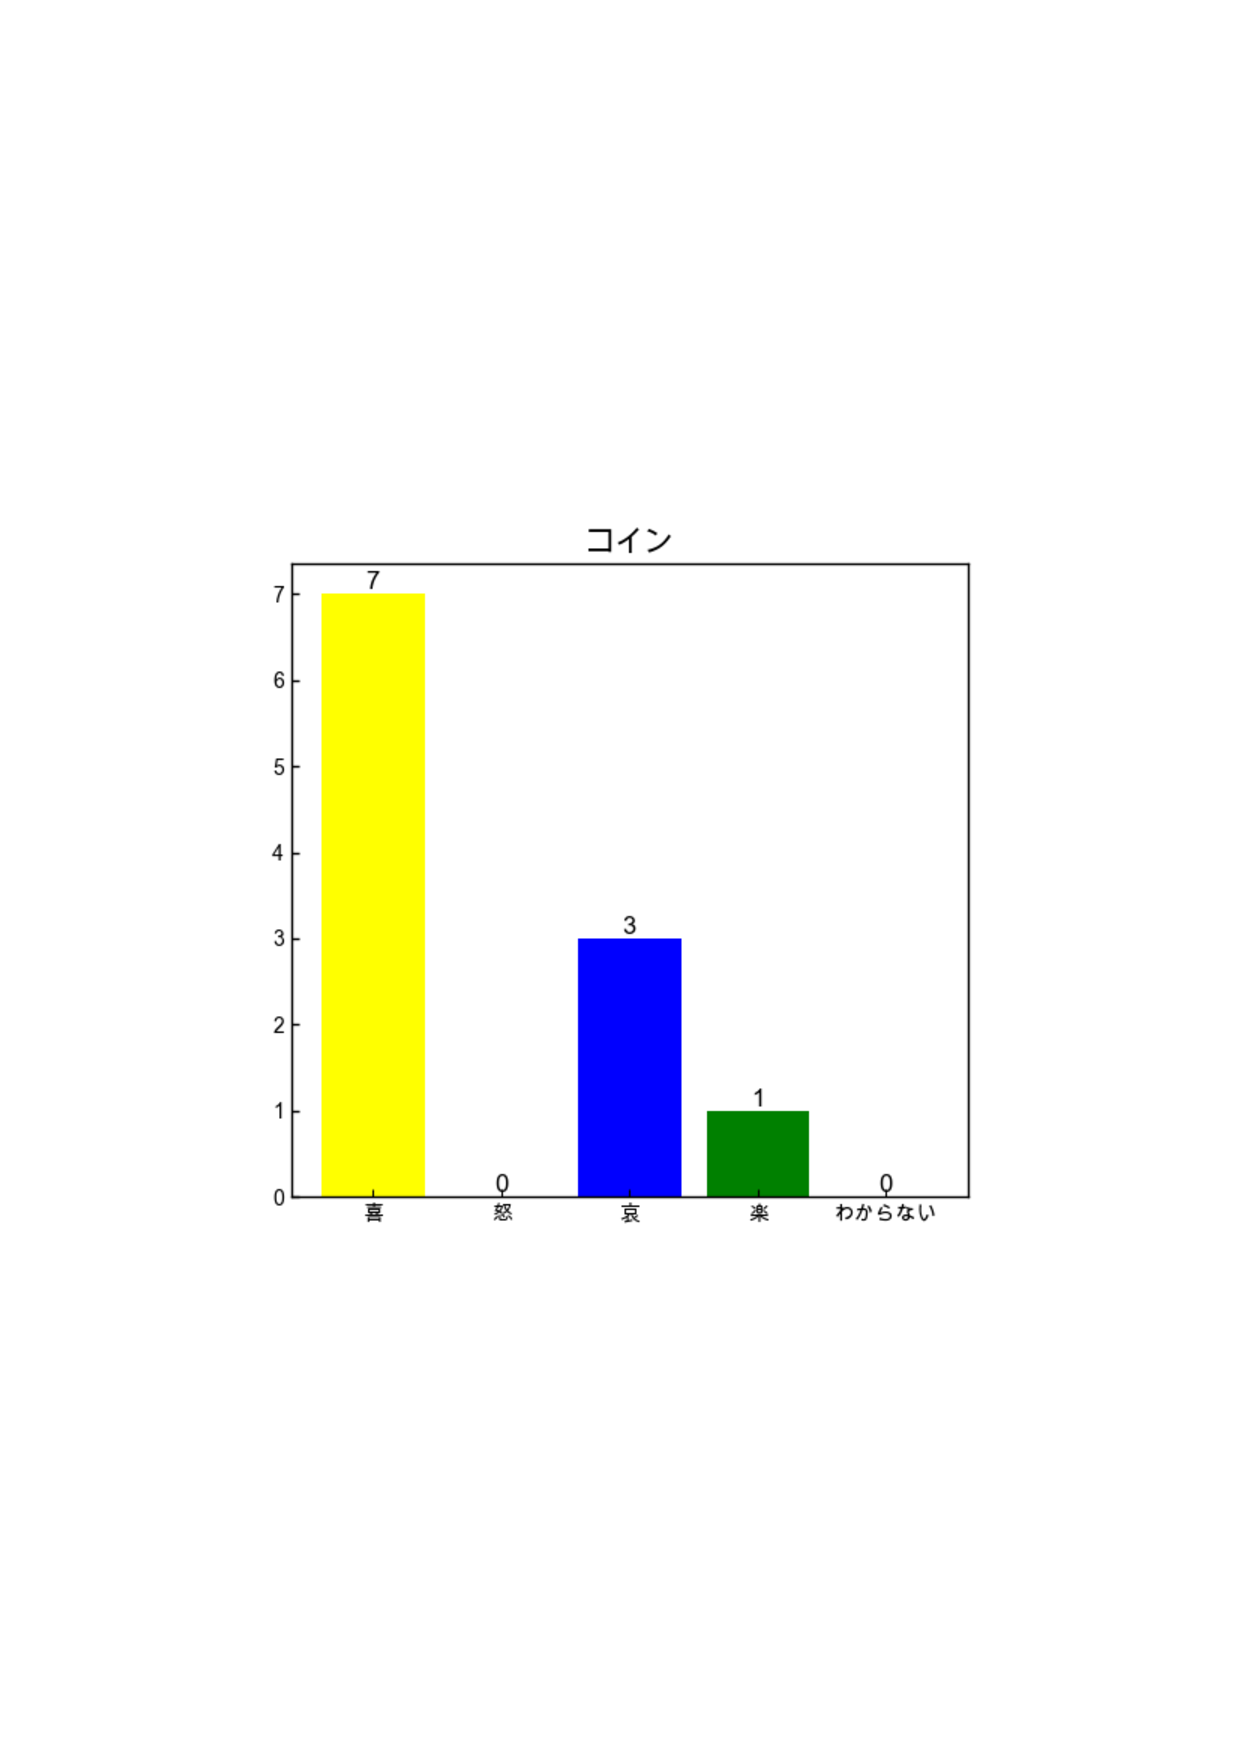
\includegraphics[width=14cm]{4320.pdf}
    \vspace{-1mm}
    \caption{歌詞 A-V-平面 第2グループ}
    \label{fig:mms}
    \vspace{5mm}
\end{figure}
第2グループから選出した「コイン」の歌詞から実験参加者3名が哀のクラスに感じたと回答した.
喜のクラスを感じたと回答した人数は7名,怒のクラスを感じたと回答した人はおらず,楽のクラスを感じたと回答した人数は1名,わからないと回答した人はいなかった.
実験参加者の多くが推定した印象を感じ取れなかったことから推定結果は不当であるといえる.
\newpage
\begin{figure}[H]
    \centering
    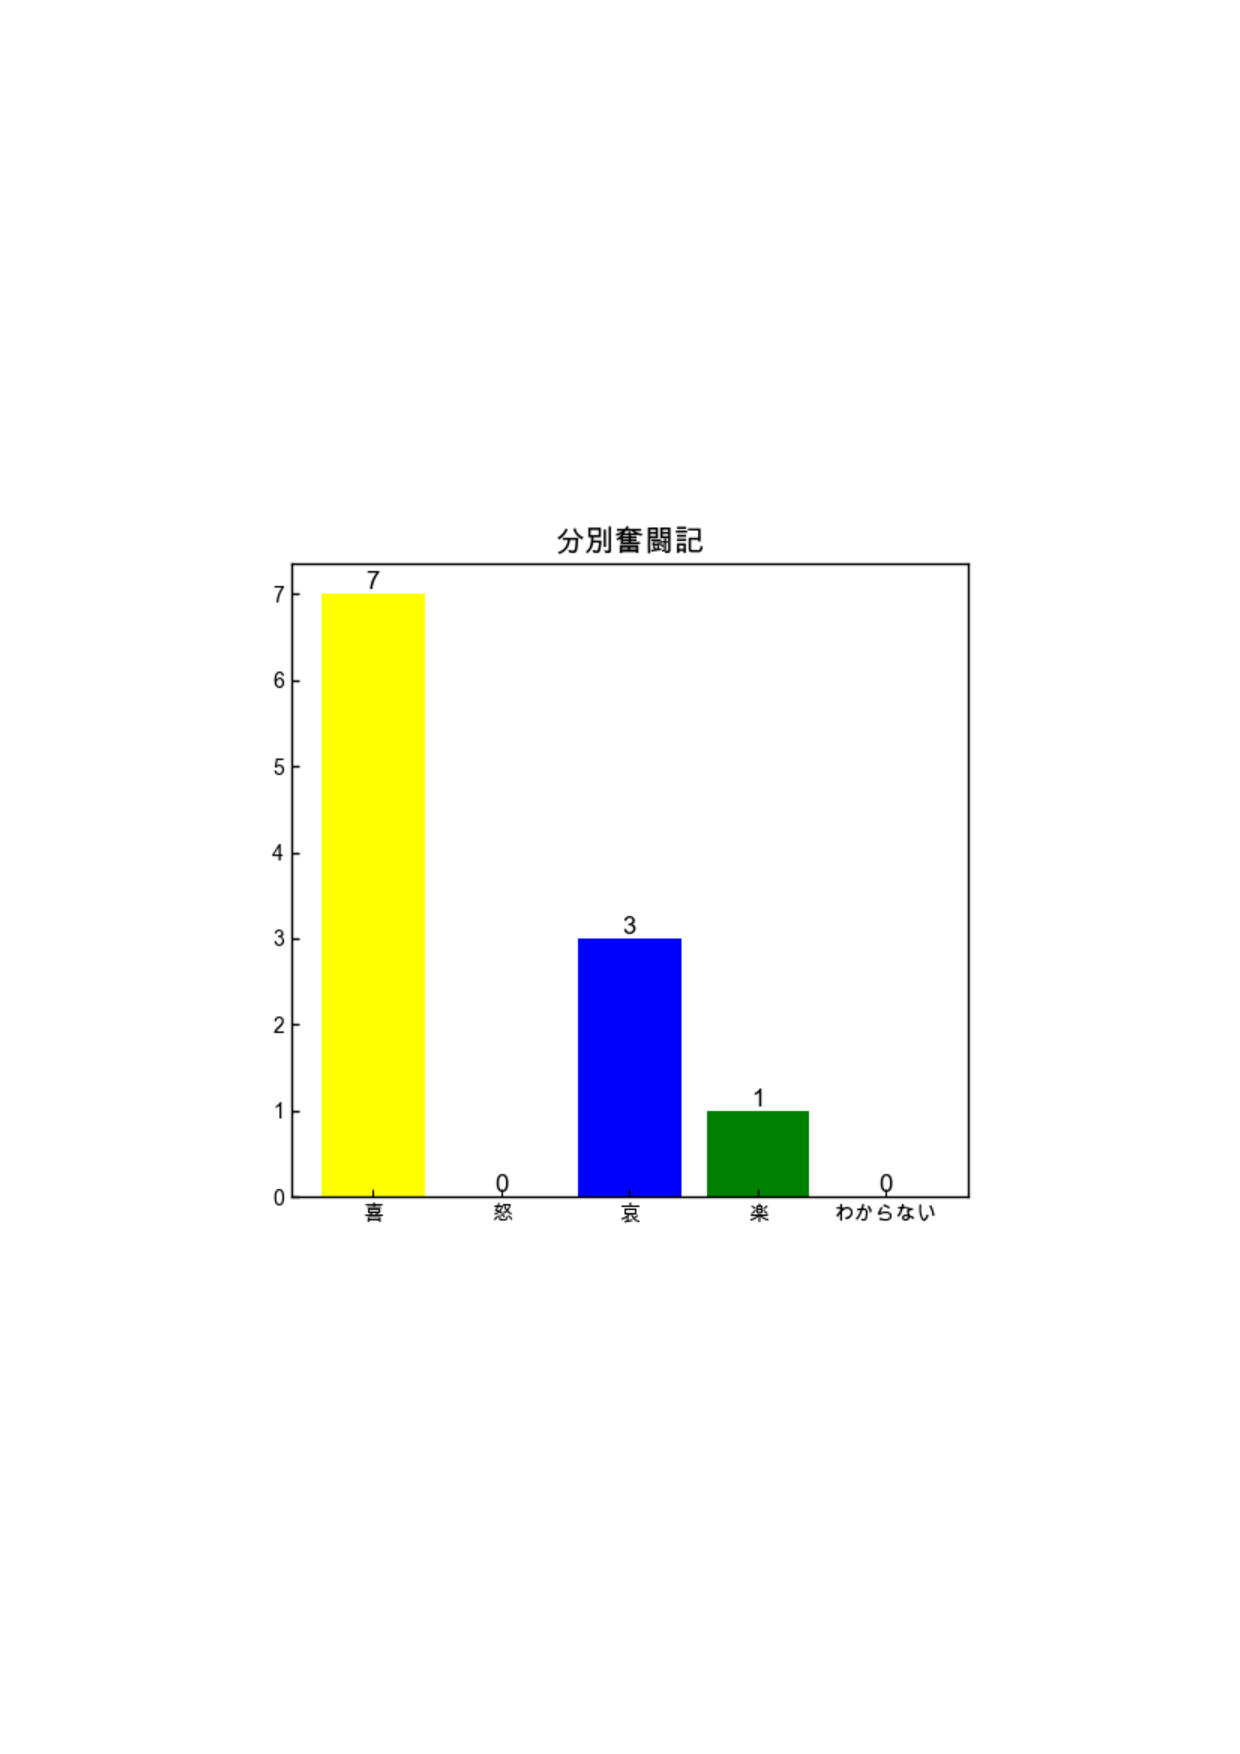
\includegraphics[width=14cm]{4321.pdf}
    \vspace{-1mm}
    \caption{歌詞 A-V-平面 第3グループ}
    \label{fig:mms}
    \vspace{5mm}
\end{figure}
第3グループから選出した「分別奮闘記」の実験結果は「コイン」の結果と同じであった.
したがって,実験参加者の多くが推定した印象を感じ取れなかったことから推定結果は不当であるといえる.
\newpage
\subsubsection{楽クラス}
楽の印象クラスにクラスタリングされた歌詞の評価結果について述べる.
第1グループから選出した「若さ故エンテレケイア」,第2グループから選出した「お互い様やん」,第3グループから選出した「シロクマ」の印象評価結果は以下の図4.10,4.11,4.12である.
\begin{figure}[H]
    \centering
    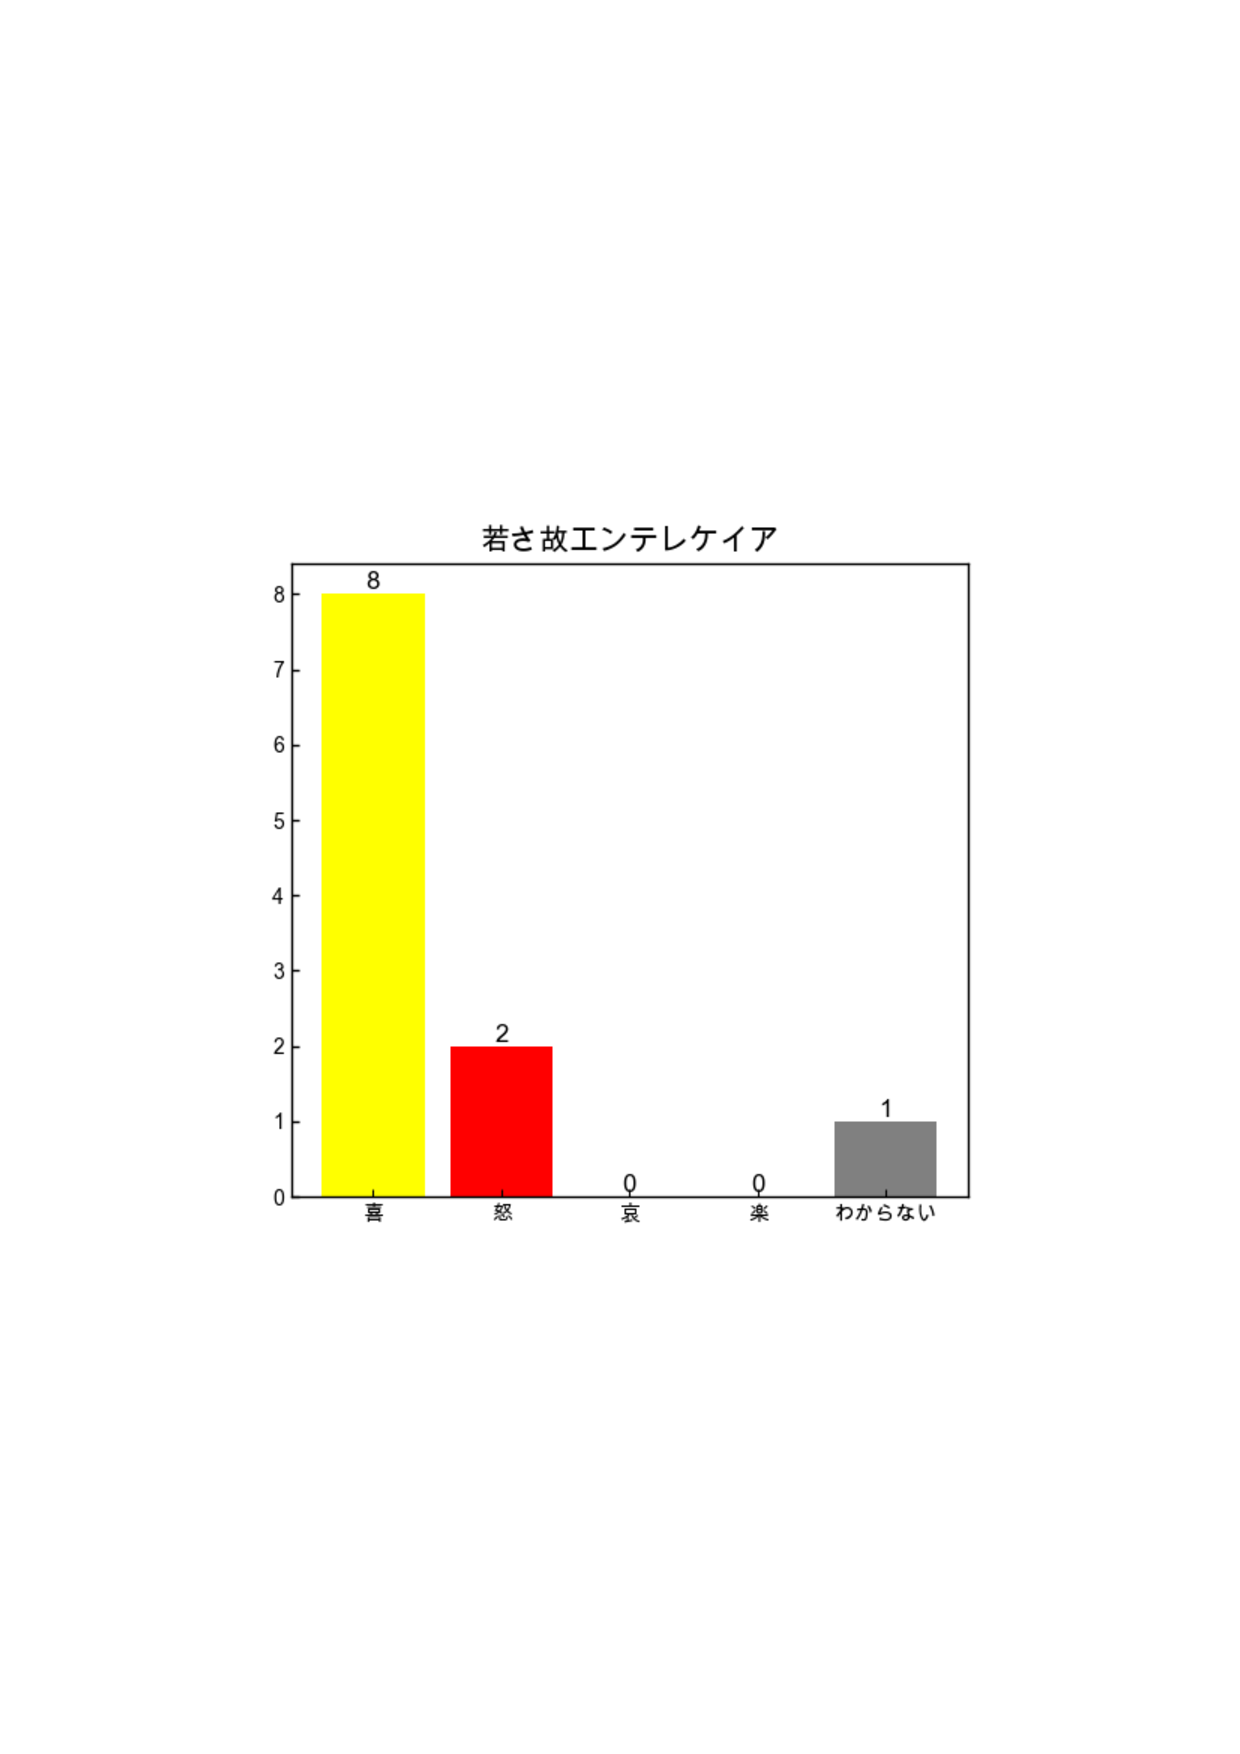
\includegraphics[width=14cm]{4322.pdf}
    \vspace{-1mm}
    \caption{歌詞 A-V+平面 第1グループ}
    \label{fig:mms}
    \vspace{5mm}
\end{figure}
第1グループから選出した「若さ故エンテレケイア」の歌詞から実験参加者0名が楽のクラスに感じたと回答した.
喜のクラスを感じたと回答した人数は8名,怒のクラスを感じたと回答した人数は2名,哀のクラスを感じたと回答した人はおらず,わからないと回答した人数は1名であった.
実験参加者が推定した印象を感じ取れなかったことから推定結果は不当であるといえる.
\newpage
\begin{figure}[H]
    \centering
    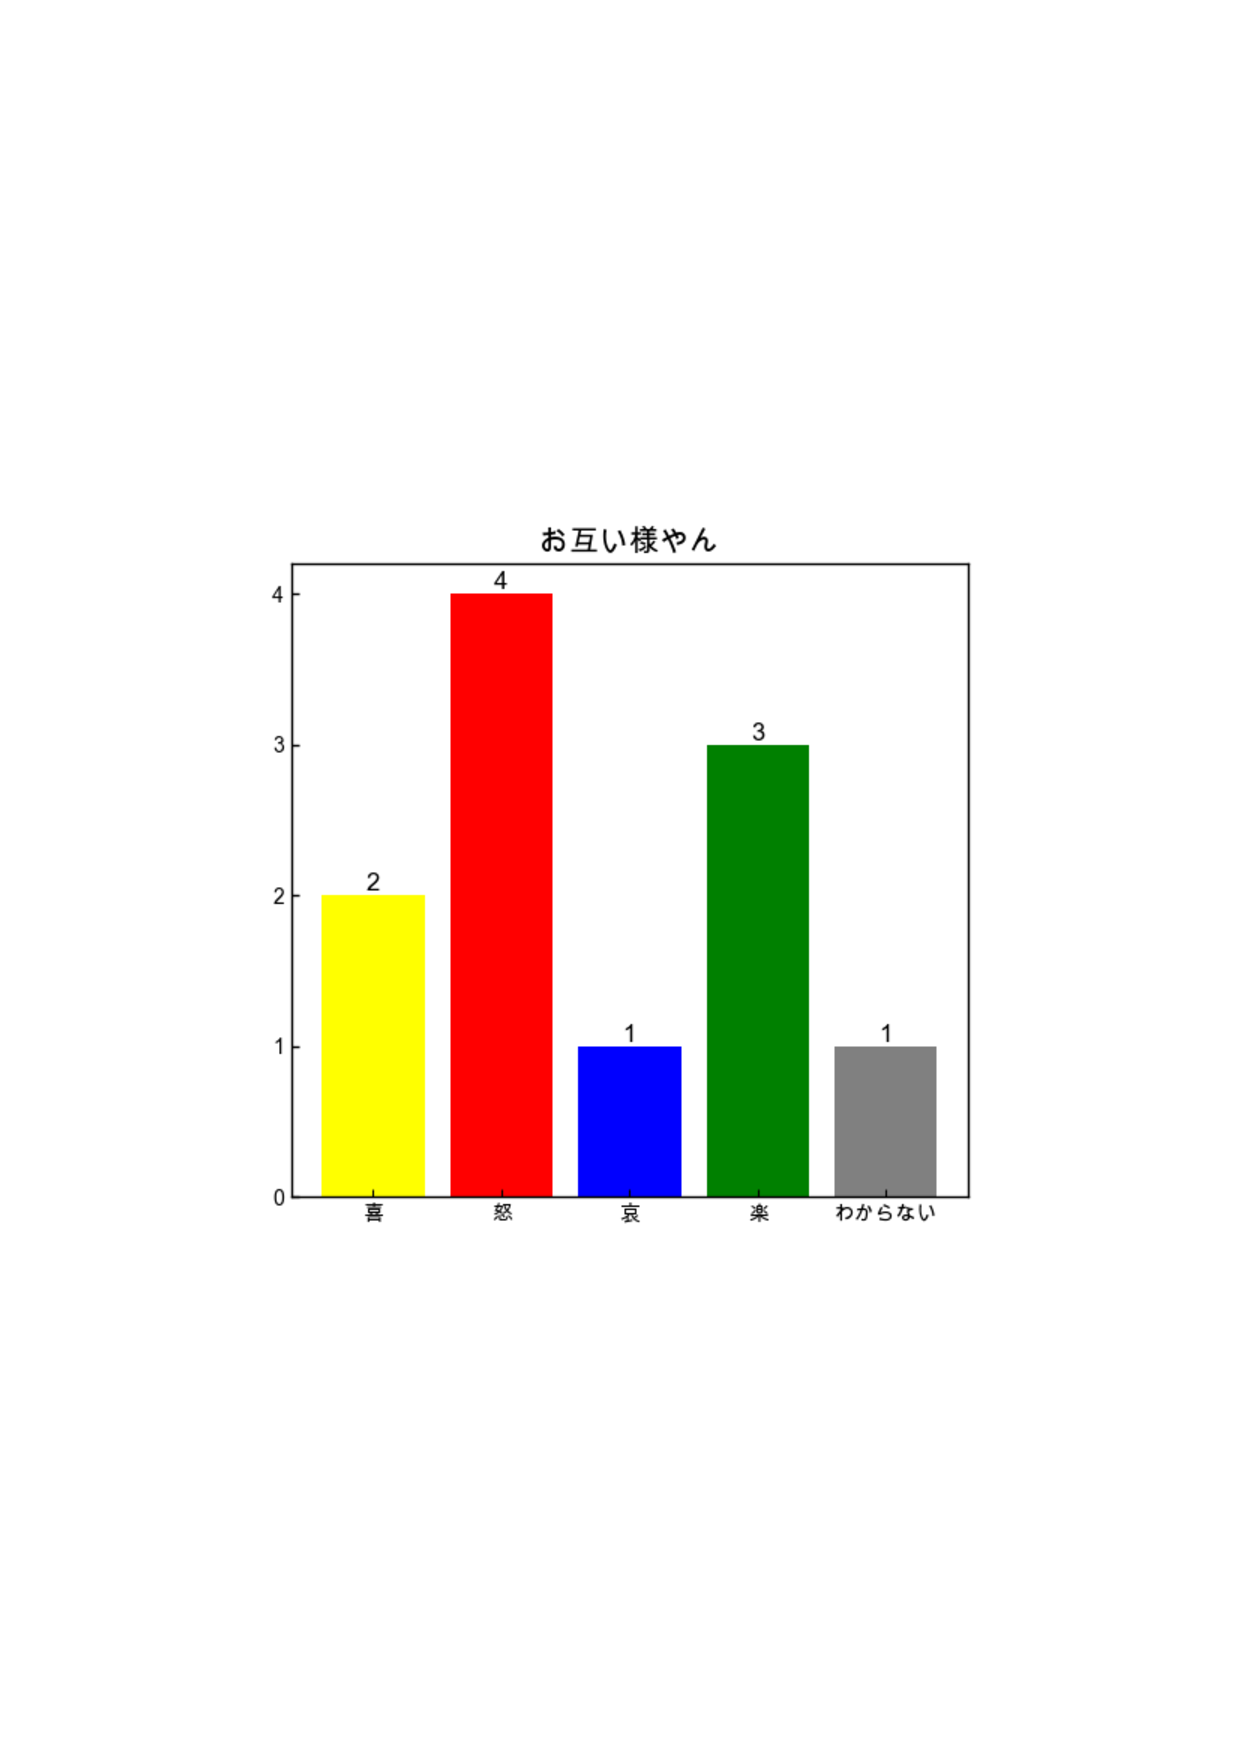
\includegraphics[width=14cm]{4323.pdf}
    \vspace{-1mm}
    \caption{歌詞 A-V+平面 第2グループ}
    \label{fig:mms}
    \vspace{5mm}
\end{figure}
第2グループから選出した「お互い様やん」の歌詞から実験参加者3名が楽のクラスに感じたと回答した.
喜のクラスを感じたと回答した人数は2名,怒のクラスを感じたと回答した人数は4名,哀のクラスを感じたと回答した人数は1名,わからないと回答した人数は1名であった.
実験参加者の多くが推定した印象を感じ取れなかったことから推定結果は不当であるといえる.
\newpage
\begin{figure}[H]
    \centering
    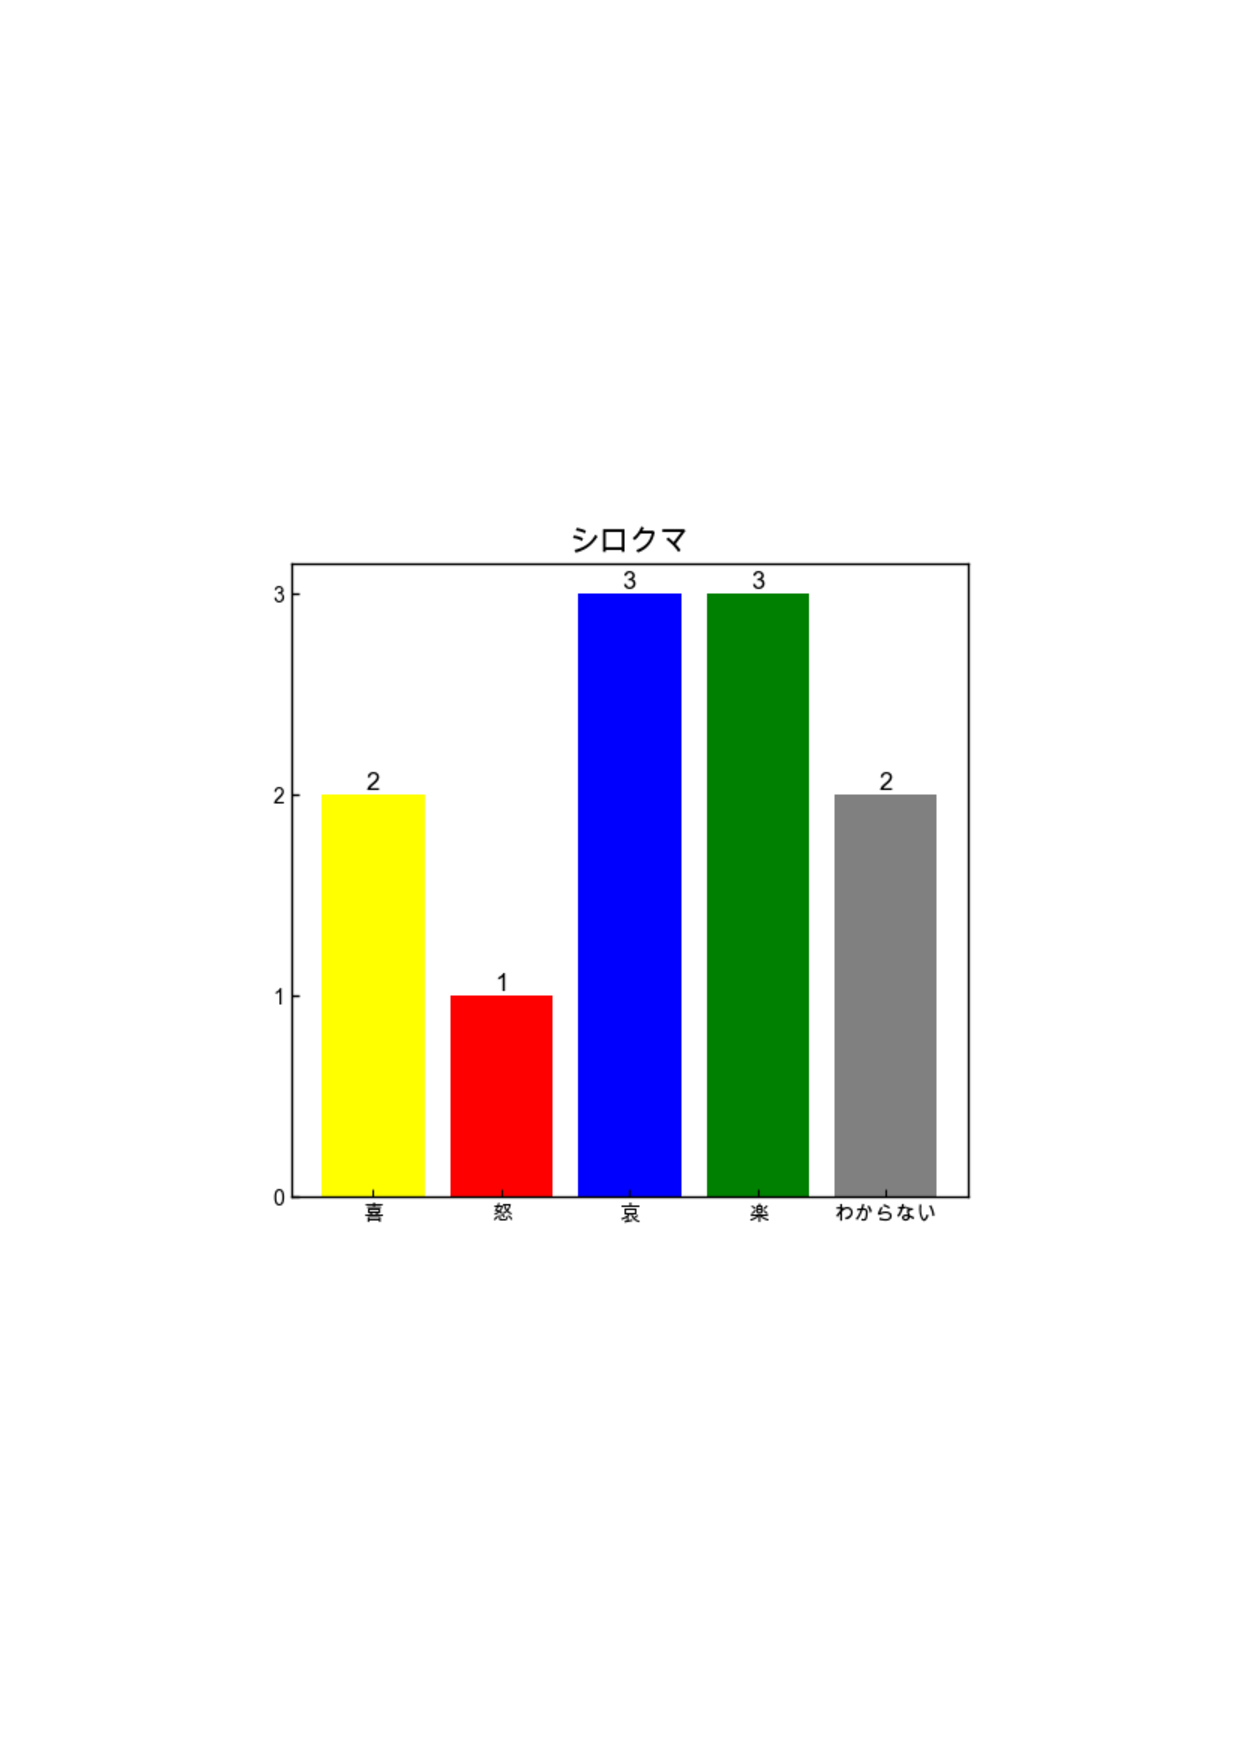
\includegraphics[width=14cm]{4324.pdf}
    \vspace{-1mm}
    \caption{歌詞 A-V+平面 第3グループ}
    \label{fig:mms}
    \vspace{5mm}
\end{figure}
第3グループから選出した「シロクマ」の歌詞から実験参加者3名が楽のクラスに感じたと回答した.
喜のクラスを感じたと回答した人数は2名,怒のクラスを感じたと回答した人数は1名,哀のクラスを感じたと回答した人数は3名,わからないと回答した人数は2名であった.
実験参加者の多くが推定した印象を感じ取れなかったことから推定結果は不当であるといえる.
\newpage
\subsection{フレーズの印象評価}
フレーズの印象評価結果について述べる.喜怒哀楽の4クラスごとに詳説する.
\subsubsection{喜クラス}
喜の印象クラスにクラスタリングされた歌詞の評価結果について述べる.
第1グループから選出した「ひとりひとり違う世界をみていくんだ」,第2グループから選出した「一石投じる生きる力」,第3グループから選出した「バタフライして」の印象評価結果は以下の図4.13,4.14,4.15である.
\begin{figure}[H]
    \centering
    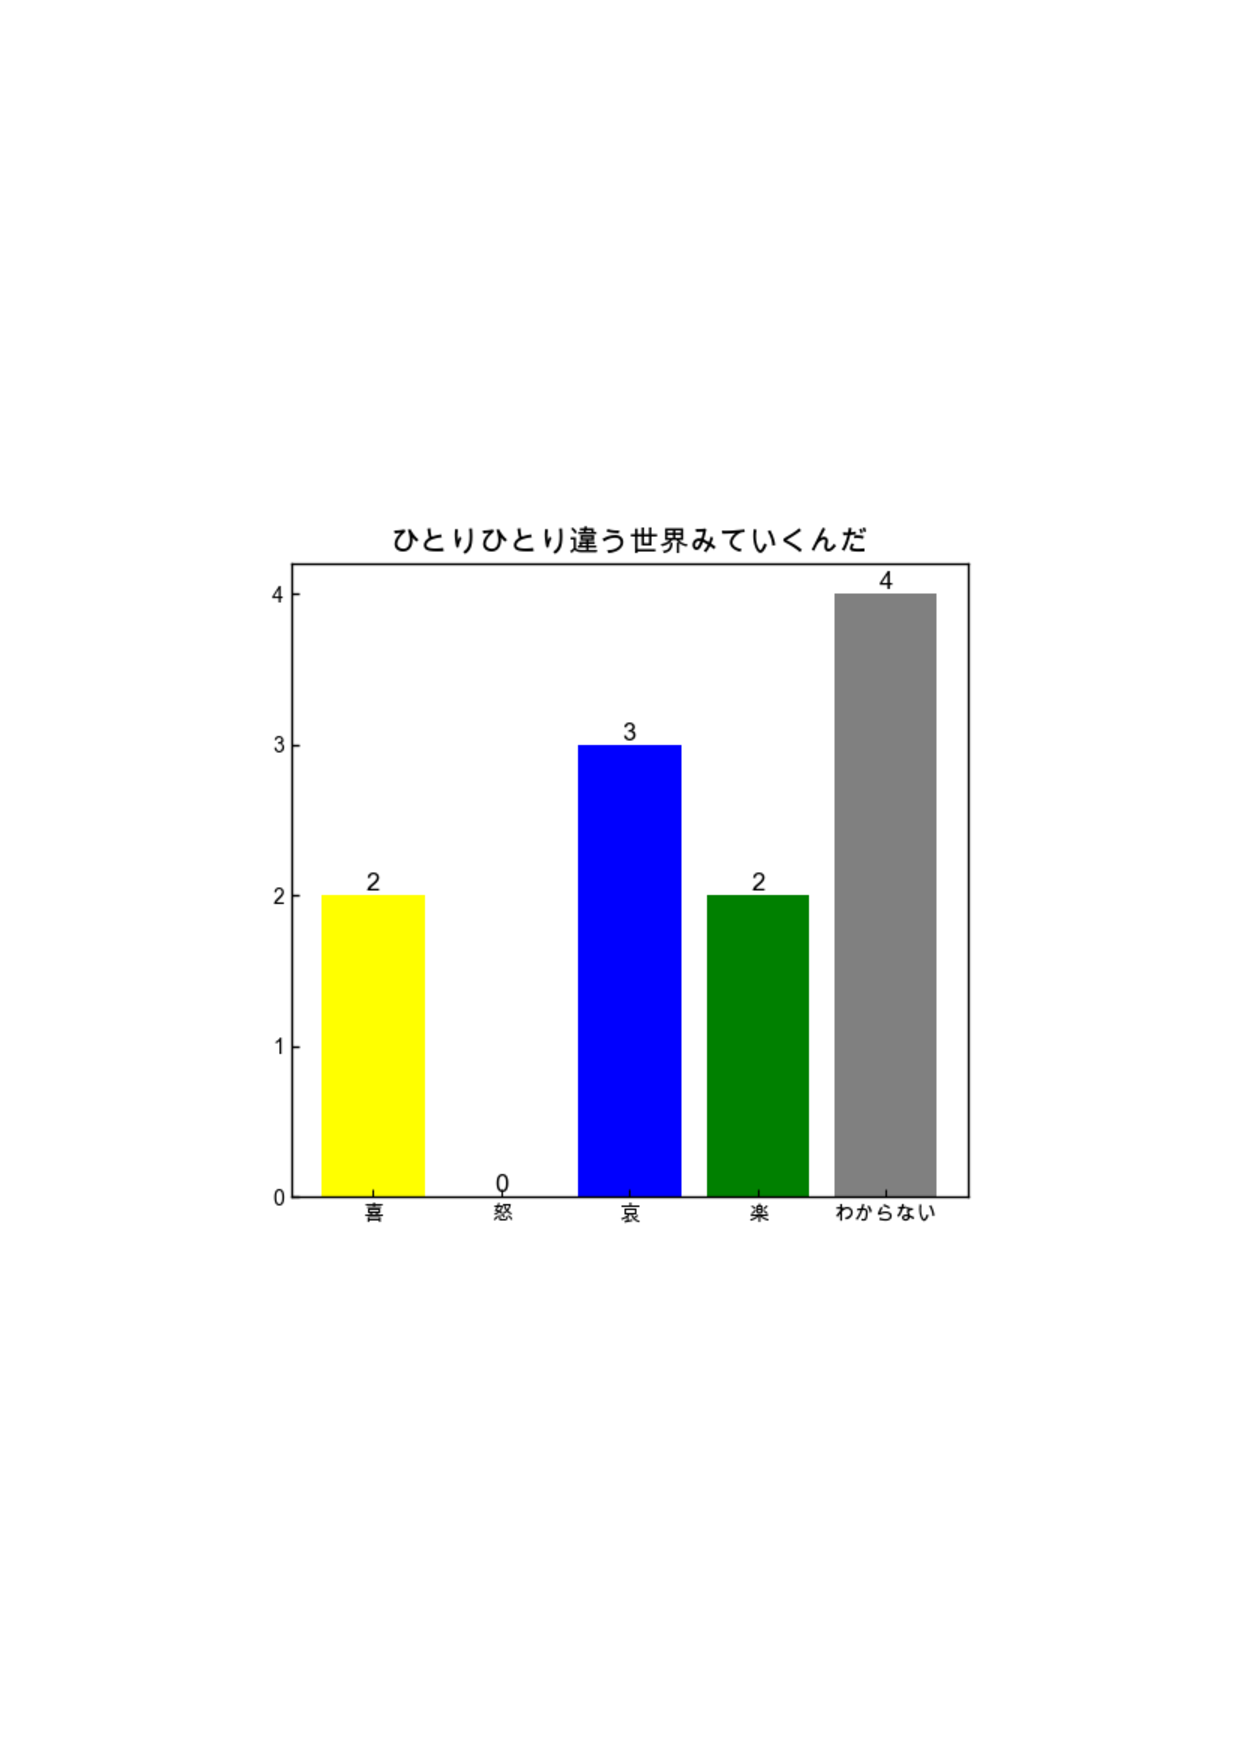
\includegraphics[width=14cm]{431.pdf}
    \vspace{-1mm}
    \caption{フレーズ A+V+平面 第1グループ}
    \label{fig:mms}
    \vspace{5mm}
\end{figure}
第1グループから選出した「ひとりひとり違う世界をみていくんだ」のフレーズから実験参加者2名が喜のクラスに感じたと回答した.
怒のクラスを感じたと回答した人はおらず,哀のクラスを感じたと回答した人数は3名,楽のクラスを感じたと回答した人数は2名,わからないと回答した人数は4名であった.
実験参加者の多くが推定した印象を感じなかったことから推定結果は不当であるといえる.
\begin{figure}[H]
    \centering
    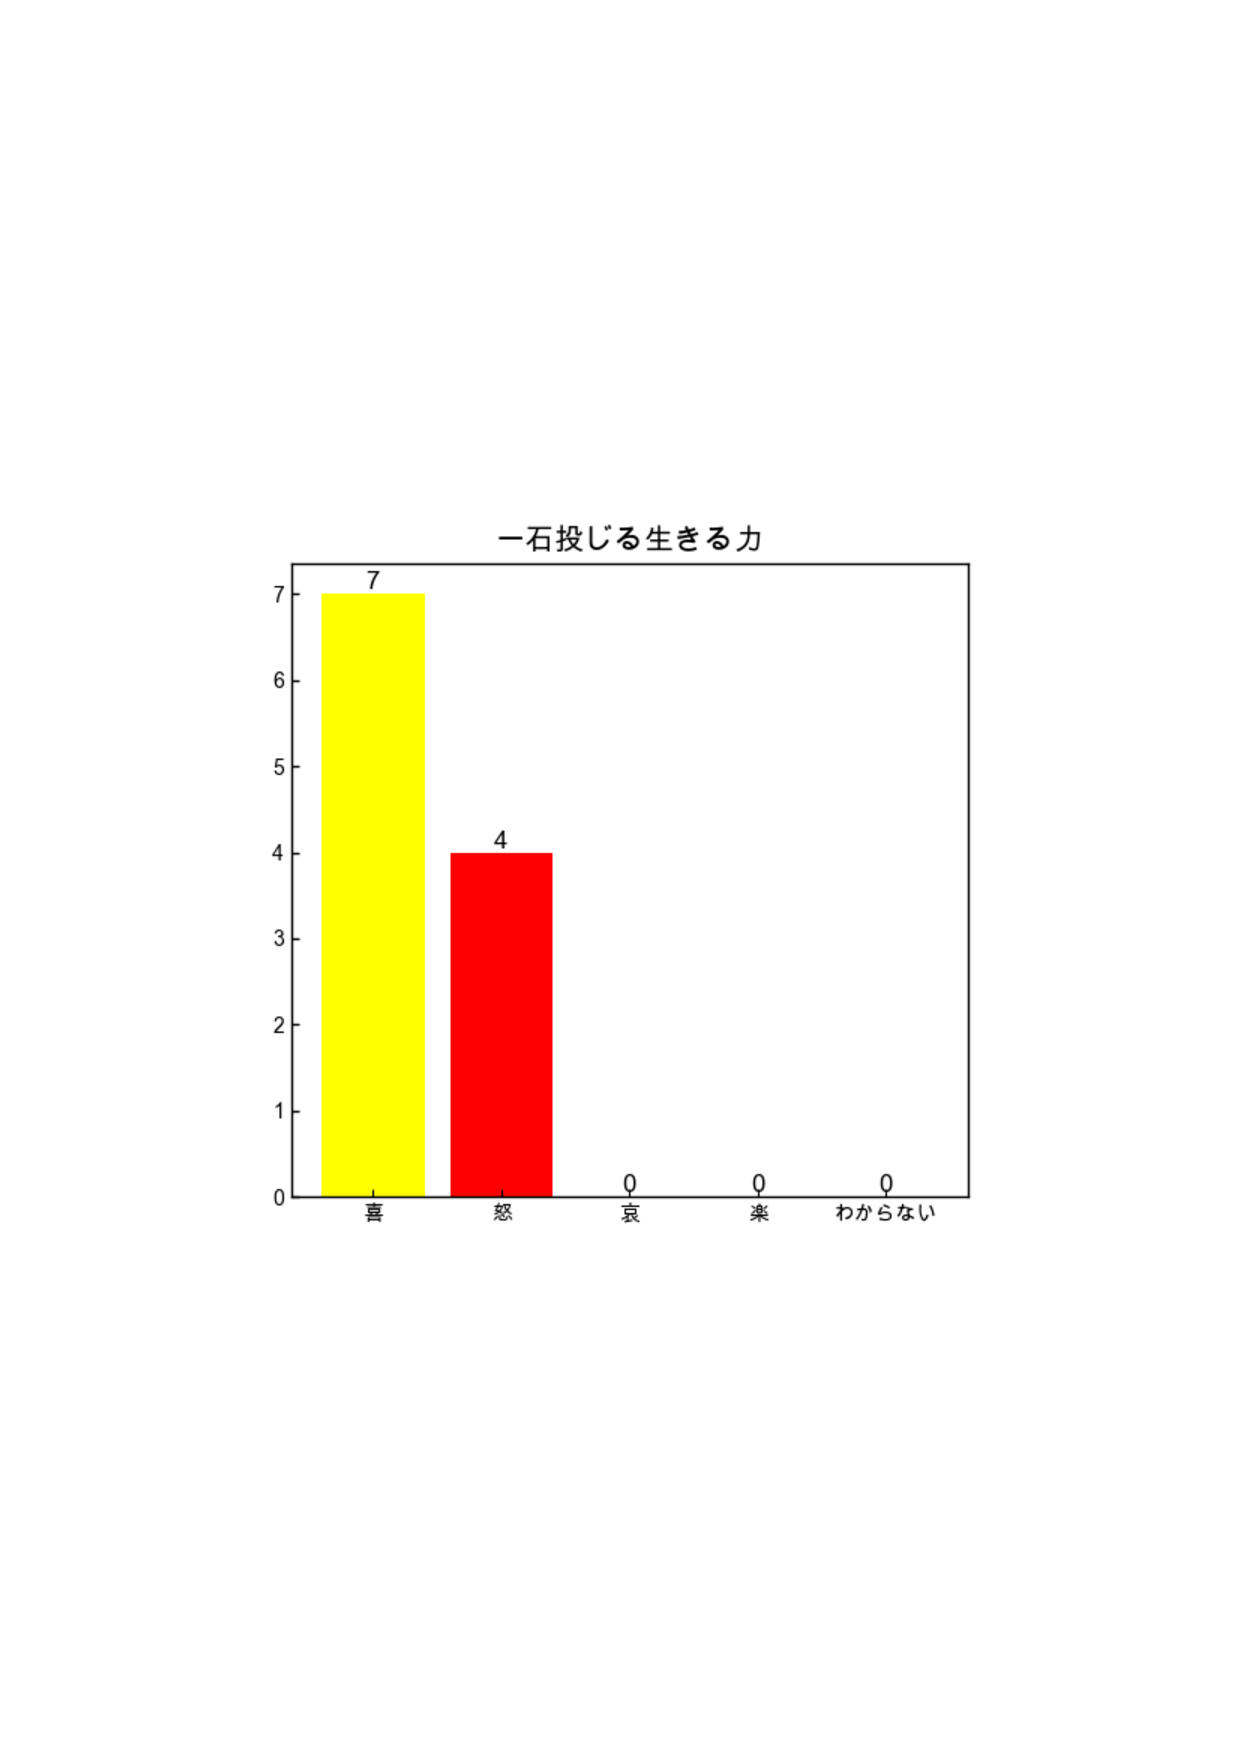
\includegraphics[width=14cm]{432.pdf}
    \vspace{-1mm}
    \caption{フレーズ A+V+平面 第2グループ}
    \label{fig:mms}
    \vspace{5mm}
\end{figure}
第2グループから選出した「一石投じる生きる力」のフレーズから実験参加者7名が喜のクラスに感じたと回答した.
怒のクラスを感じたと回答した人数は4名,哀と楽のクラスを感じたまたはわからないと回答した人はいなかった.
実験参加者の多くが推定した印象を感じたことから推定結果は妥当であるといえる.
\newpage
\begin{figure}[H]
    \centering
    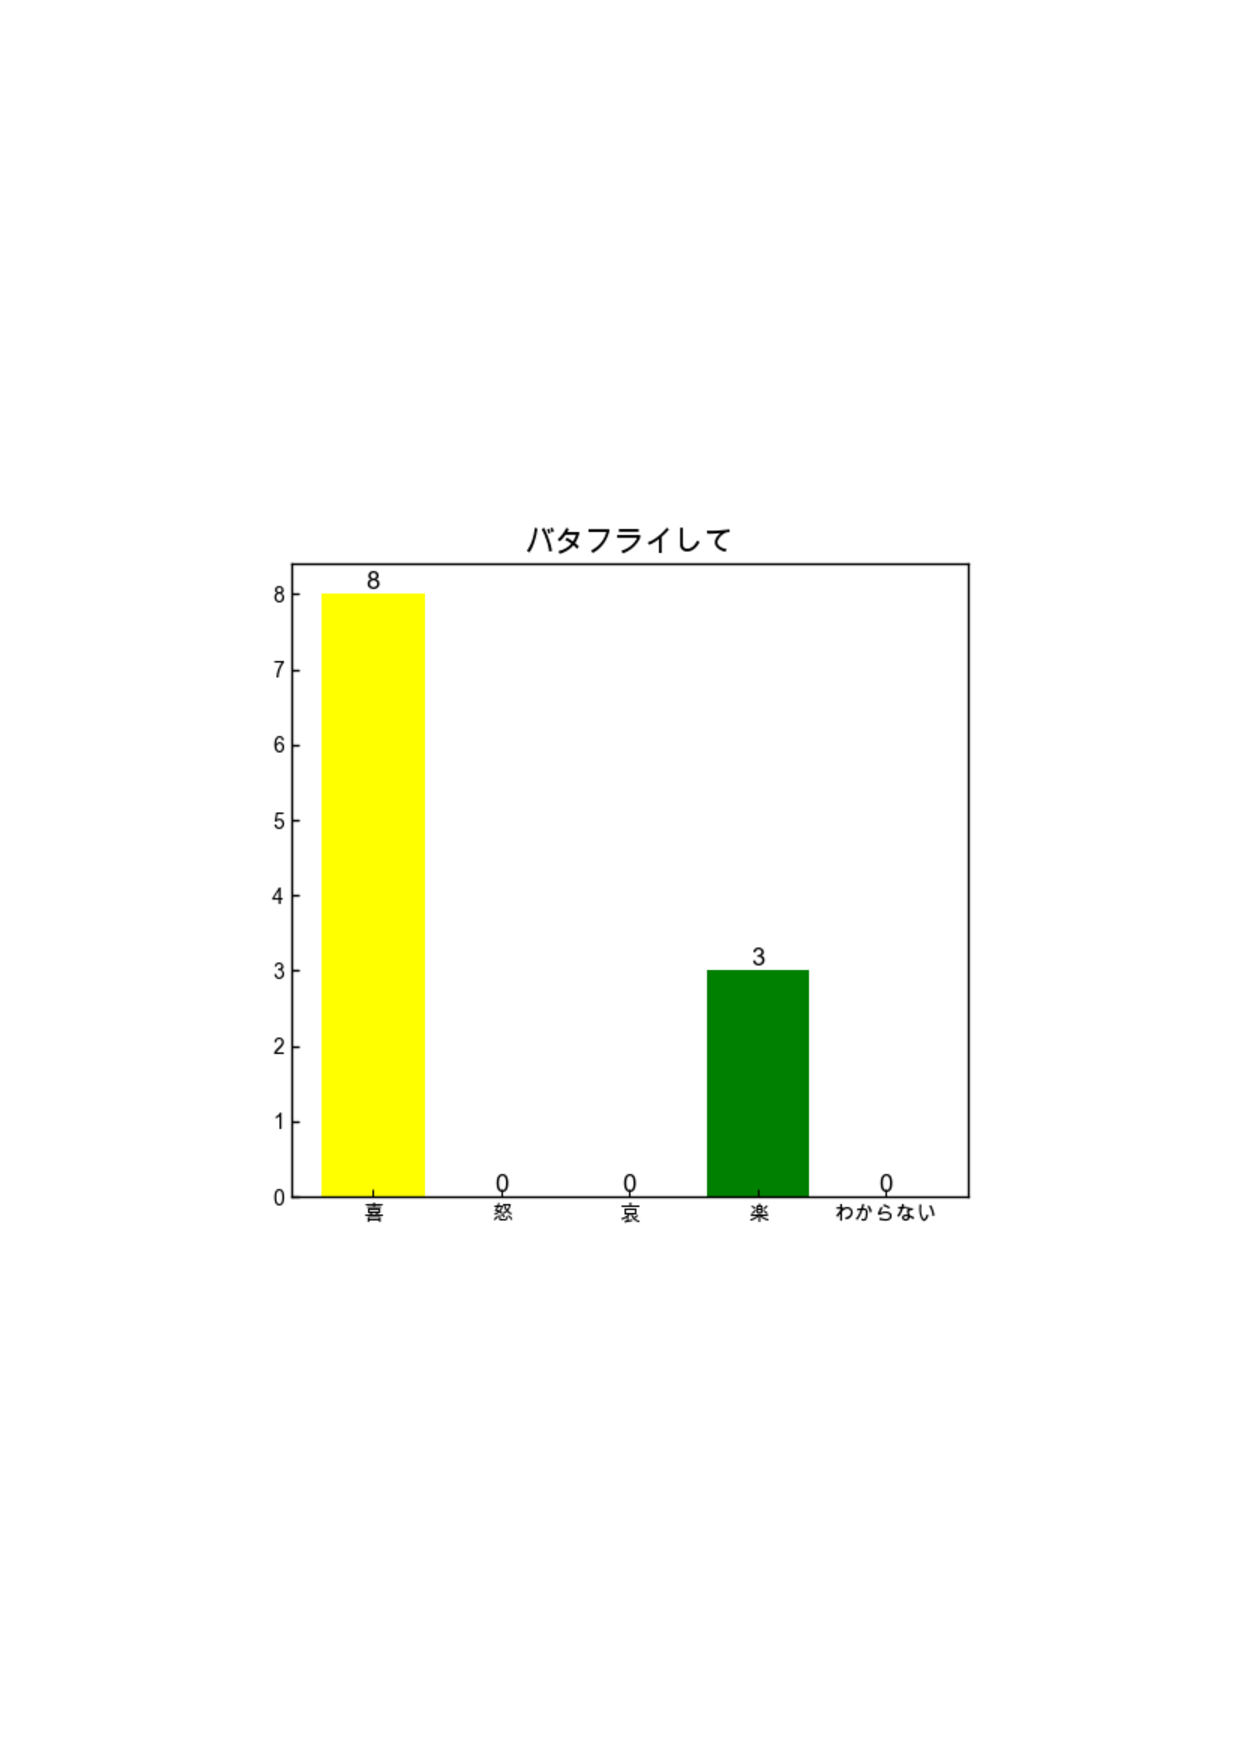
\includegraphics[width=14cm]{433.pdf}
    \vspace{-1mm}
    \caption{フレーズ A+V+平面 第3グループ}
    \label{fig:mms}
    \vspace{5mm}
\end{figure}
第3グループから選出した「バタフライして」のフレーズから実験参加者8名が喜のクラスに感じたと回答した.
楽のクラスを感じたと回答した人数は3名,哀と怒のクラスを感じたまたはわからないと回答した人はいなかった.
実験参加者の多くが推定した印象を感じたことから推定結果は妥当であるといえる.
\newpage
\subsubsection{怒クラス}
怒の印象クラスにクラスタリングされた歌詞の評価結果について述べる.
第1グループから選出した「演じる意味はどこもブレたまま」,第2グループから選出した「二つ並んだ影法師の手」,第3グループから選出した「マイクホン争奪戦」の印象評価結果は以下の図4.16,4.17,4.18である.
\begin{figure}[H]
    \centering
    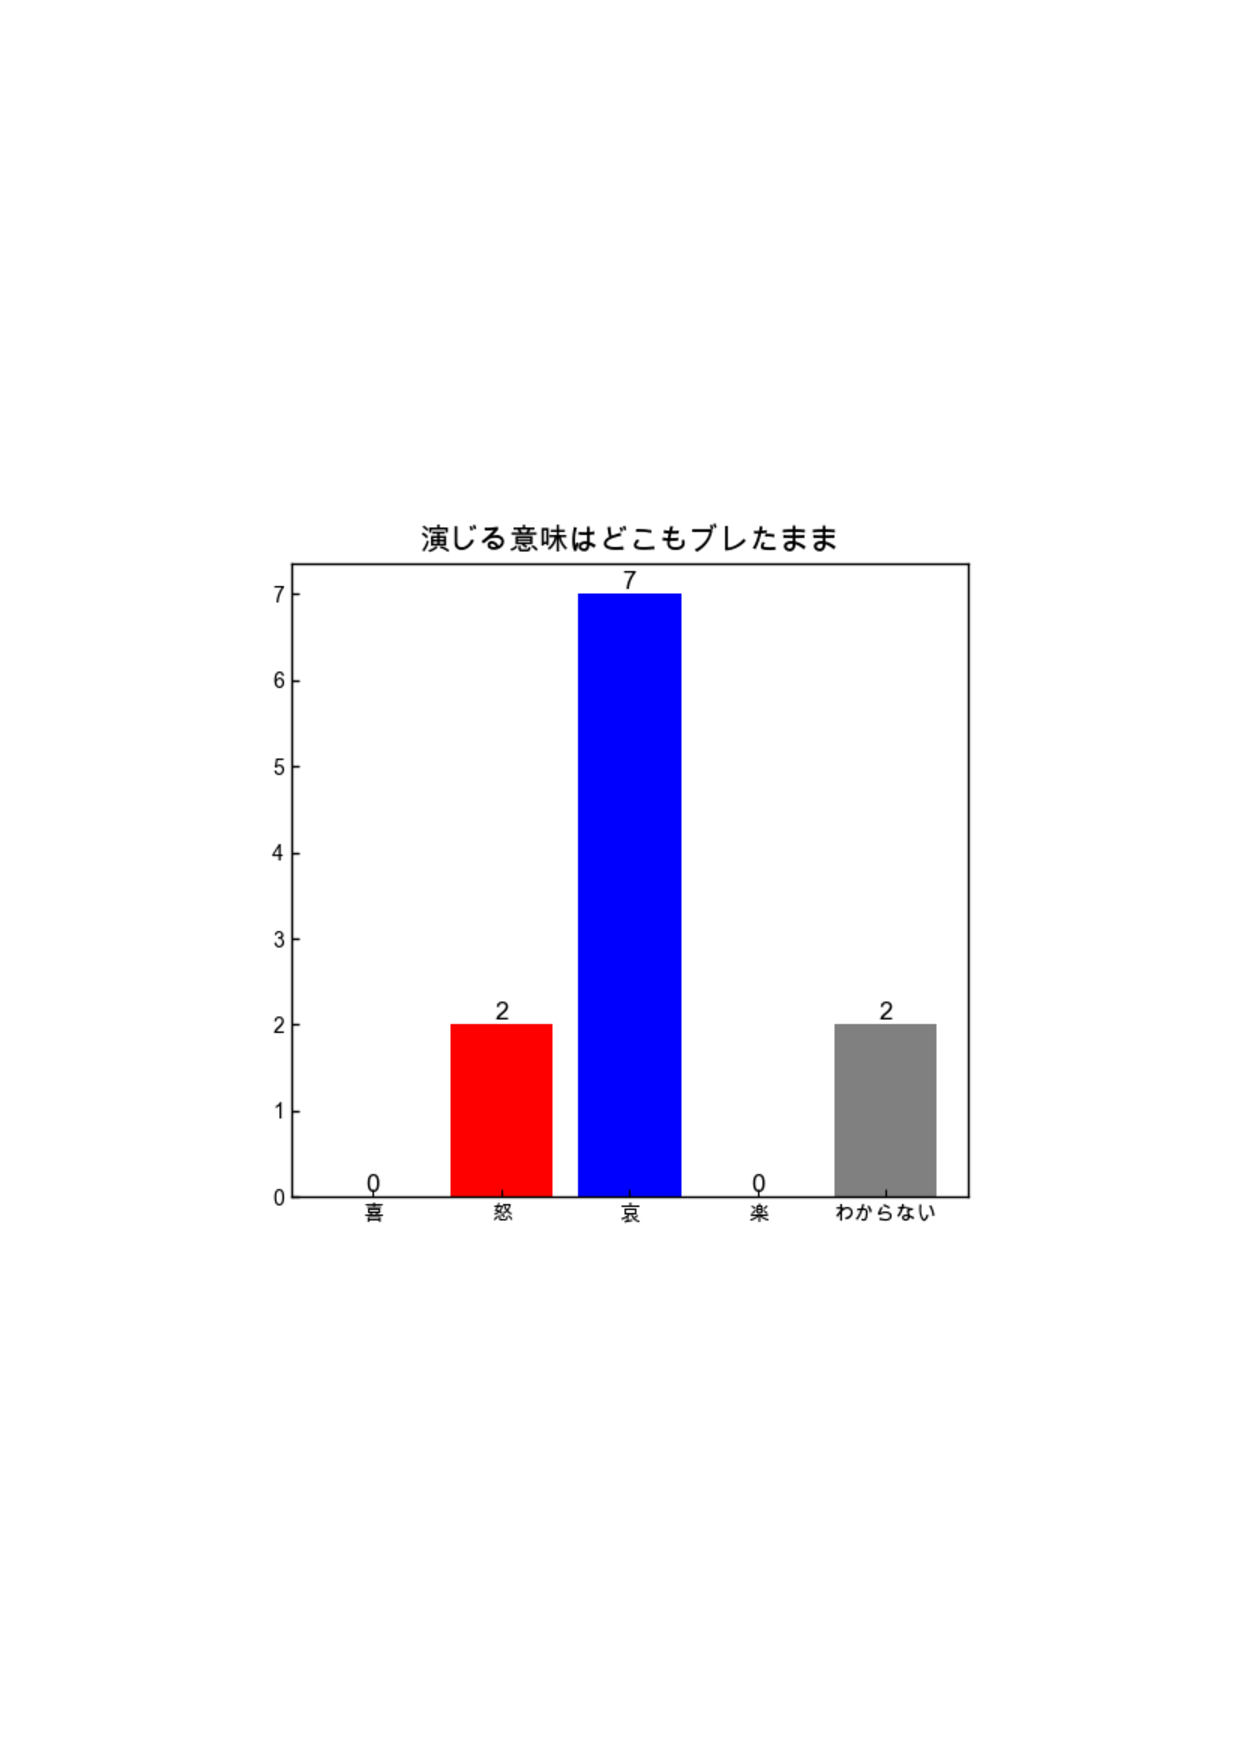
\includegraphics[width=14cm]{434.pdf}
    \vspace{-1mm}
    \caption{フレーズ A+V-平面 第1グループ}
    \label{fig:mms}
    \vspace{5mm}
\end{figure}
第1グループから選出した「演じる意味はどこもブレたまま」のフレーズから実験参加者2名が怒のクラスに感じたと回答した.
哀のクラスを感じたと回答した人数は7名,喜と楽のクラスを感じたおらず,わからないと回答した人数は2名であった.
実験参加者の多くが推定した印象を感じていないことから推定結果は不当であるといえる.
\newpage
\begin{figure}[H]
    \centering
    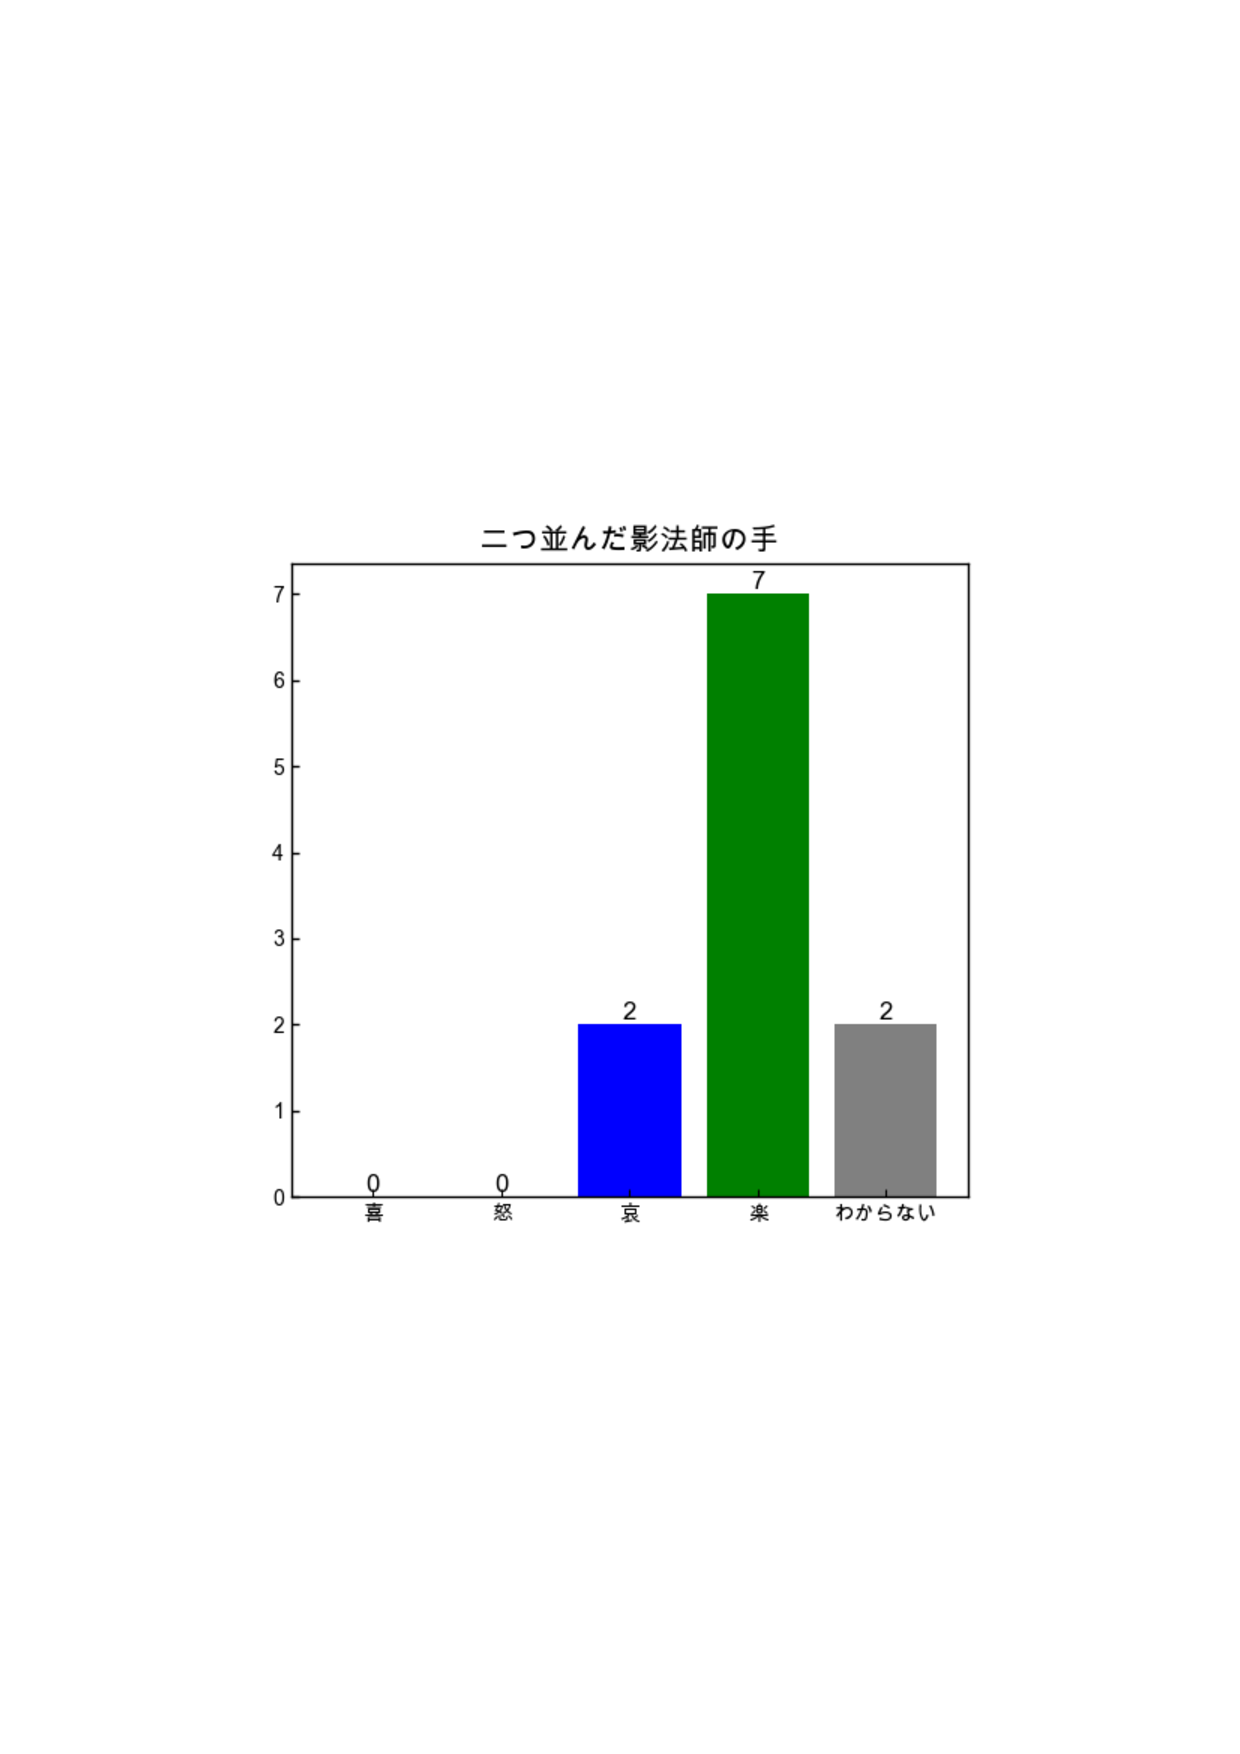
\includegraphics[width=14cm]{435.pdf}
    \vspace{-1mm}
    \caption{フレーズ A+V-平面 第2グループ}
    \label{fig:mms}
    \vspace{5mm}
\end{figure}
第2グループから選出した「二つ並んだ影法師の手」のフレーズから実験参加者0名が怒のクラスに感じたと回答した.
喜のクラスを感じた人はおらず,哀のクラスを感じたと回答した人数は2名,楽のクラスを感じたと回答した人数は7名,わからないと回答した人数は2名であった.
実験参加者の多くが推定した印象を感じていないことから推定結果は不当であるといえる.
\newpage
\begin{figure}[H]
    \centering
    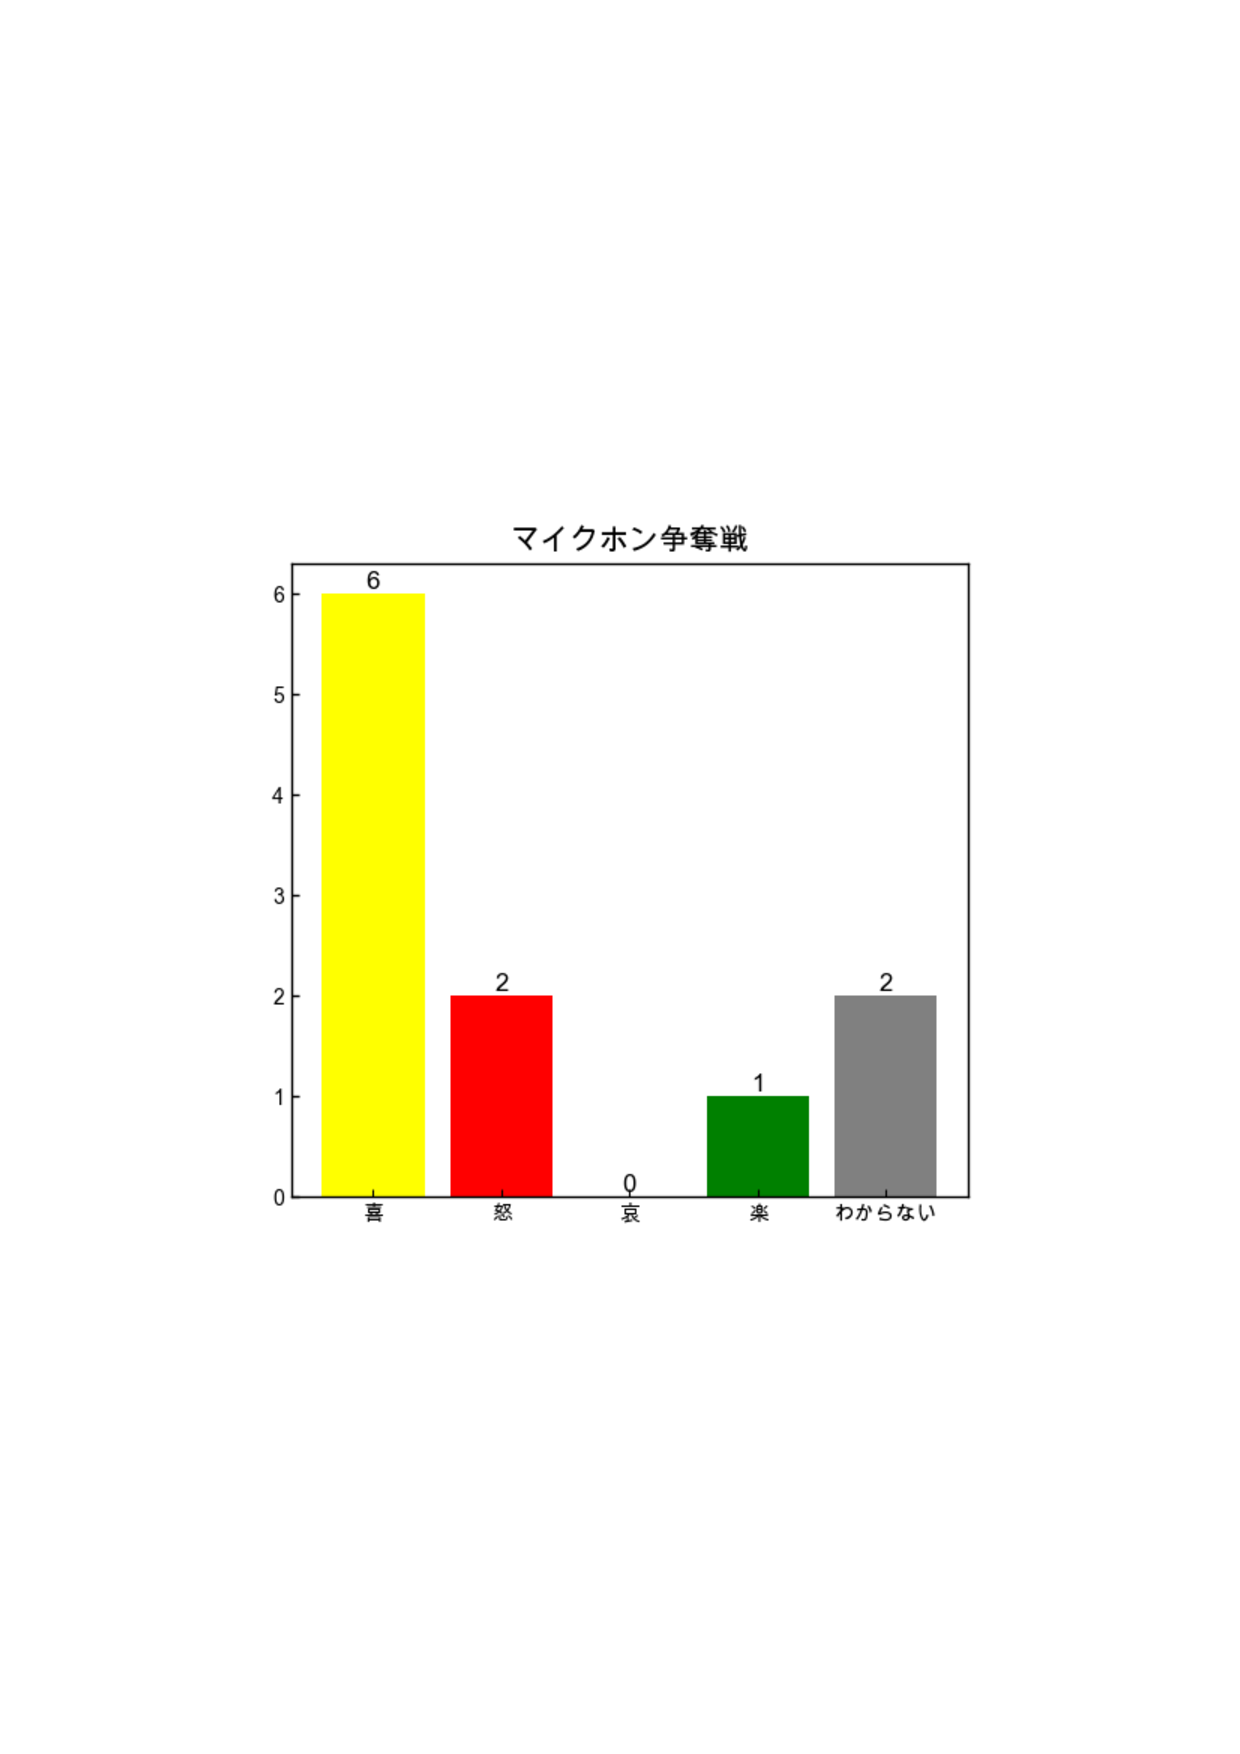
\includegraphics[width=14cm]{436.pdf}
    \vspace{-1mm}
    \caption{フレーズ A+V-平面 第3グループ}
    \label{fig:mms}
    \vspace{5mm}
\end{figure}
第3グループから選出した「マイクホン争奪戦」のフレーズから実験参加者2名が怒のクラスに感じたと回答した.
喜のクラスを感じた人数は6名,哀のクラスを感じたと回答した人はおらず,楽のクラスを感じたと回答した人数は1名,わからないと回答した人数は2名であった.
実験参加者の多くが推定した印象を感じていないことから推定結果は不当であるといえる.
\newpage
\subsubsection{哀クラス}
哀の印象クラスにクラスタリングされた歌詞の評価結果について述べる.
第1グループから選出した「私を捨てたあなたは馬鹿で」,第2グループから選出した「あなたを苦しめたことでしょう」,第3グループから選出した「昨今のあなたは鼻につくわ」の印象評価結果は以下の図4.19,4.20,4.21である.
\begin{figure}[H]
    \centering
    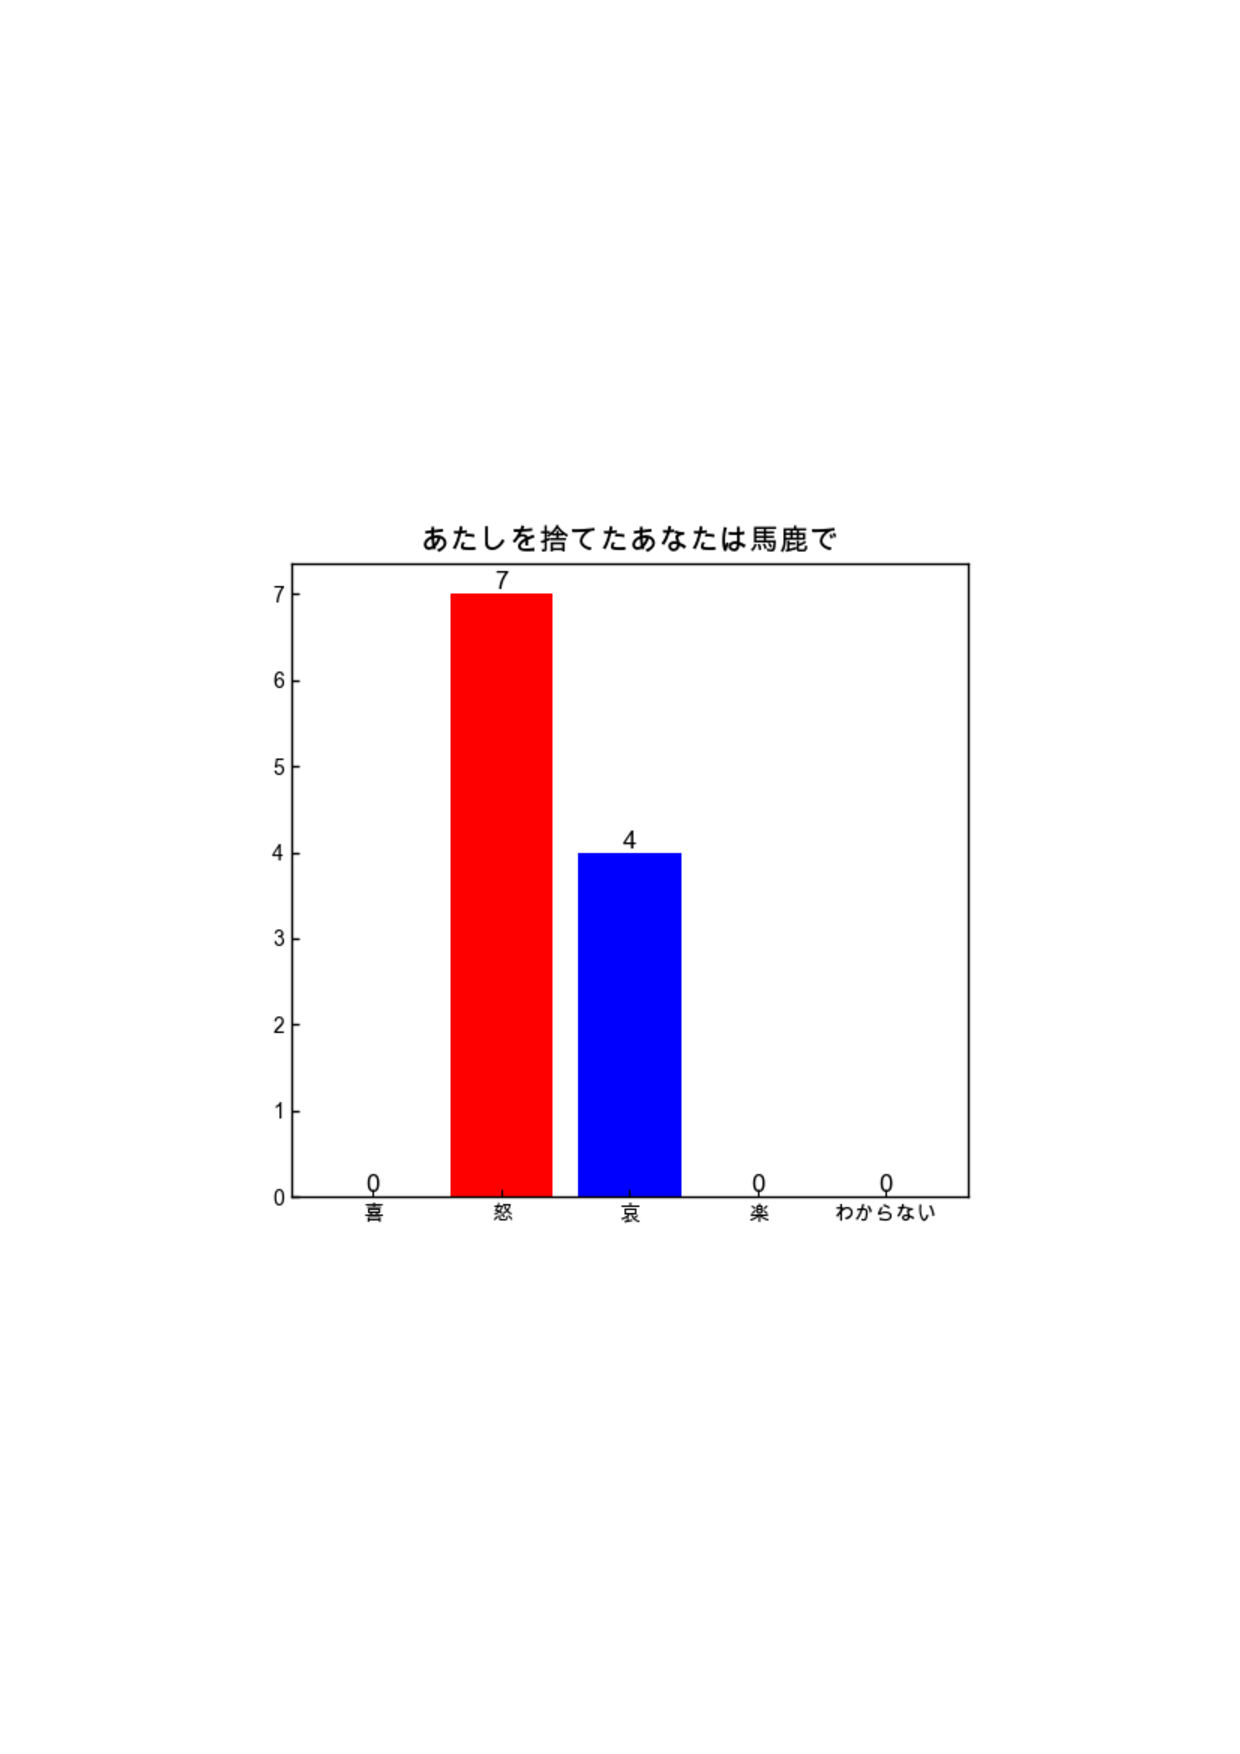
\includegraphics[width=14cm]{437.pdf}
    \vspace{-1mm}
    \caption{フレーズ A-V-平面 第1グループ}
    \label{fig:mms}
    \vspace{5mm}
\end{figure}
第1グループから選出した「私を捨てたあなたは馬鹿で」のフレーズから実験参加者4名が哀のクラスに感じたと回答した.
怒のクラスを感じたと回答した人数は7名,喜と楽のクラスを感じた,またはわからないと回答した人はいなかった.
実験参加者の多くが推定した印象を感じていないことから推定結果は不当であるといえる.
\newpage
\begin{figure}[H]
    \centering
    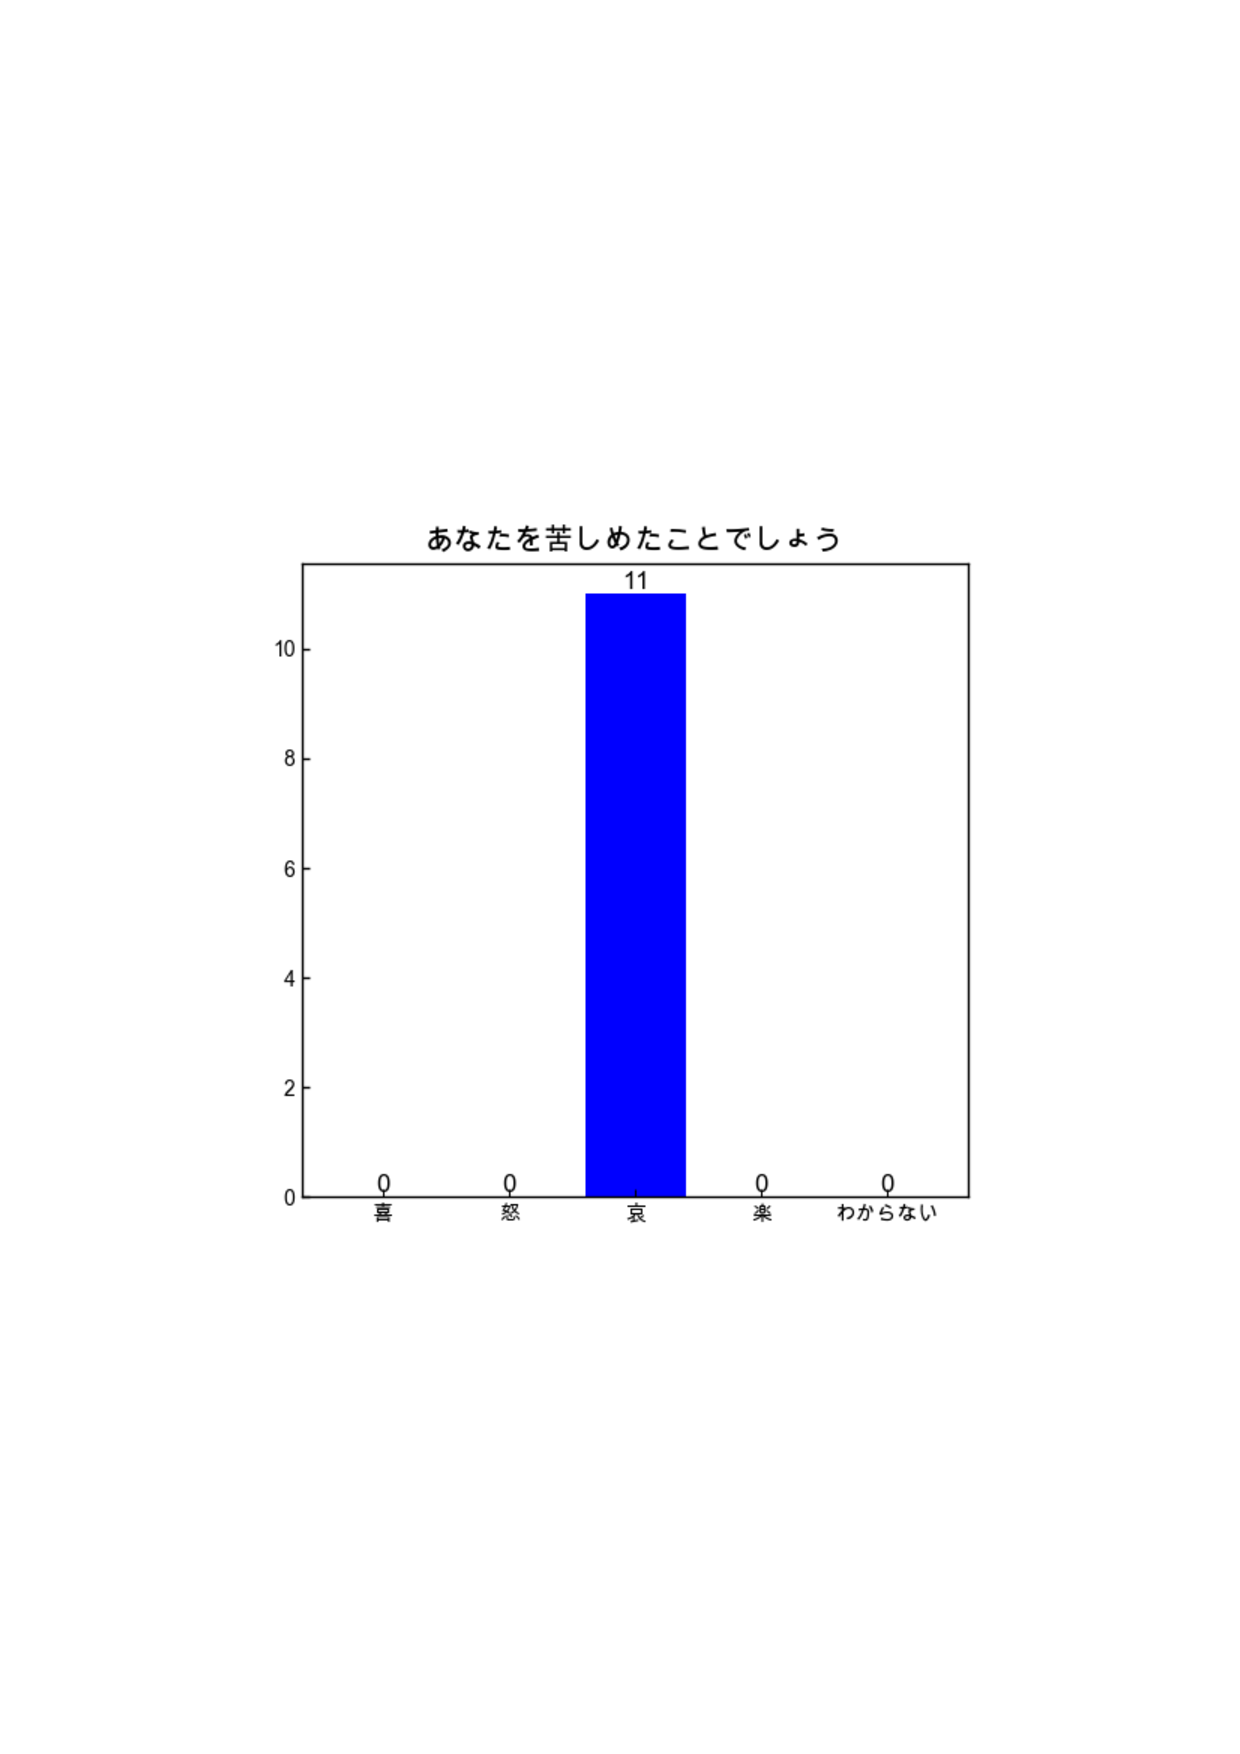
\includegraphics[width=14cm]{438.pdf}
    \vspace{-1mm}
    \caption{フレーズ A-V-平面 第2グループ}
    \label{fig:mms}
    \vspace{5mm}
\end{figure}
第2グループから選出した「あなたを苦しめたことでしょう」のフレーズから実験参加者11名全員が哀のクラスに感じたと回答した.
実験参加者全員が推定した印象を感じたことから推定結果は妥当であるといえる.
\newpage
\begin{figure}[H]
    \centering
    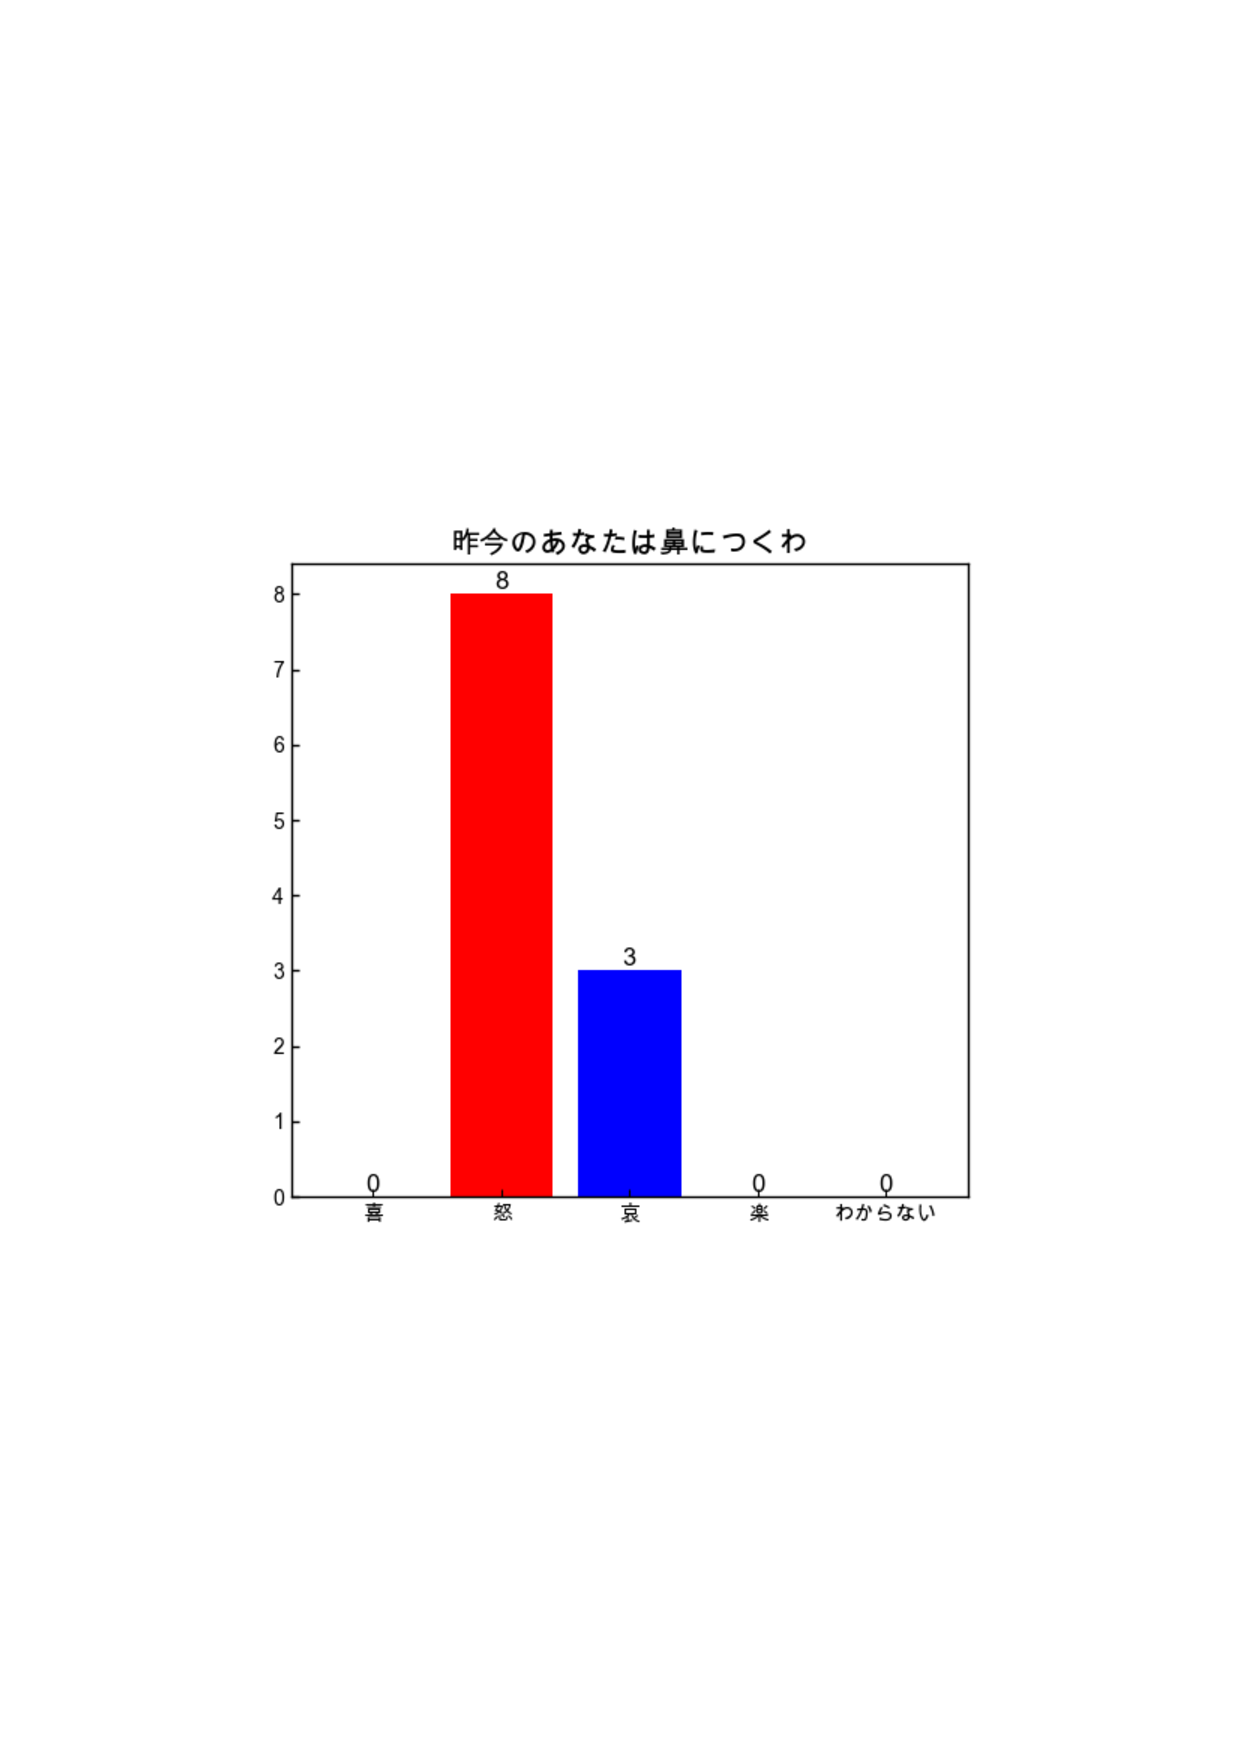
\includegraphics[width=14cm]{439.pdf}
    \vspace{-1mm}
    \caption{フレーズ A-V-平面 第3グループ}
    \label{fig:mms}
    \vspace{5mm}
\end{figure}
第3グループから選出した「昨今のあなたは鼻につくわ」のフレーズから実験参加者3名が哀のクラスに感じたと回答した.
怒のクラスを感じたと回答した人数は8名,喜と楽のクラスを感じた,またはわからないと回答した人はいなかった.
実験参加者の多くが推定した印象を感じていないことから推定結果は不当であるといえる.
\newpage
\subsubsection{楽クラス}
楽の印象クラスにクラスタリングされた歌詞の評価結果について述べる.
第1グループから選出した「浮かぶ月にやさしく響いては消えていった」,第2グループから選出した「染まる真っ赤なギロチン」,第3グループから選出した「しぶといトラウマも全部払おう」の印象評価結果は以下の図4.22,4.23,4.24である.
\begin{figure}[H]
    \centering
    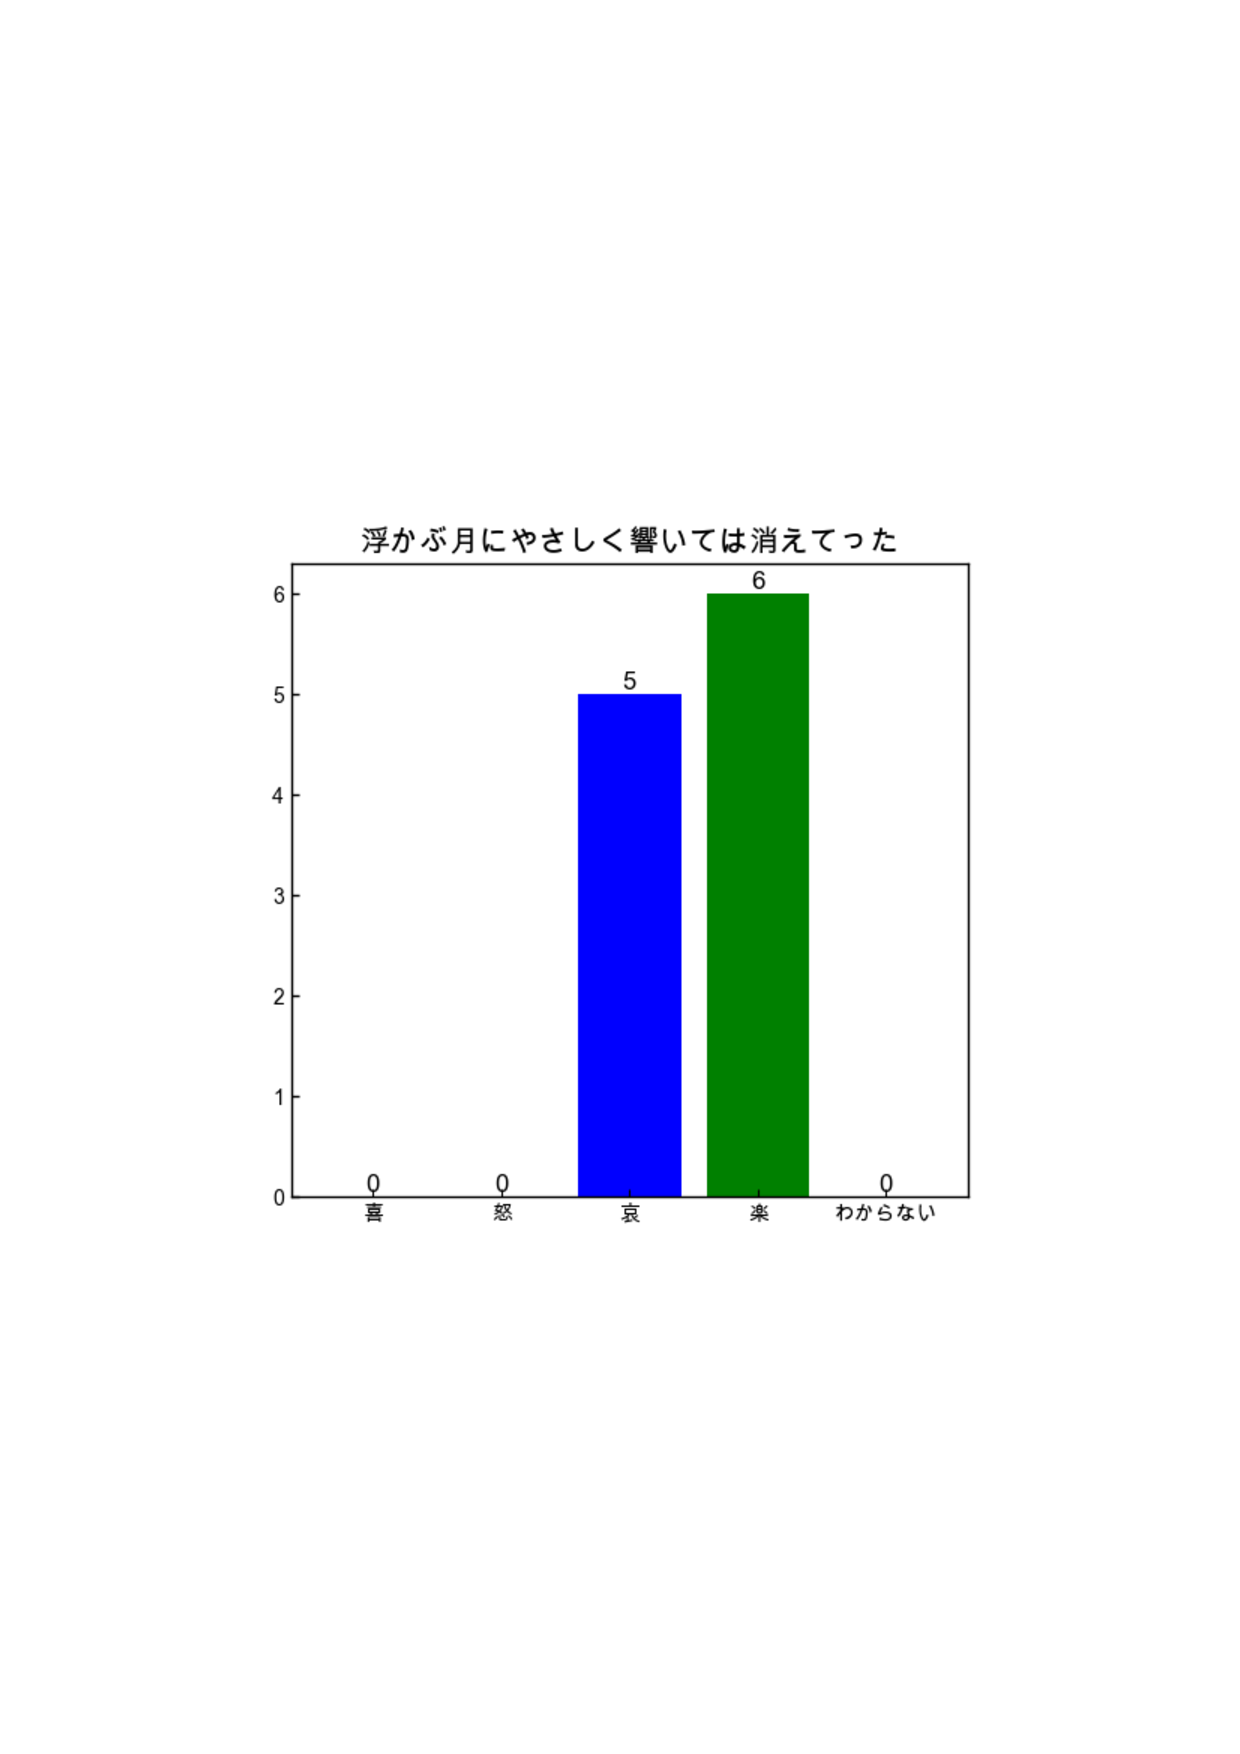
\includegraphics[width=14cm]{4310.pdf}
    \vspace{-1mm}
    \caption{フレーズ A-V+平面 第1グループ}
    \label{fig:mms}
    \vspace{5mm}
\end{figure}
第1グループから選出した「浮かぶ月にやさしく響いては消えていった」のフレーズから実験参加者6名が楽のクラスに感じたと回答した.
哀のクラスを感じたと回答した人数は5名,喜と怒のクラスを感じた,またはわからないと回答した人はいなかった.
実験参加者の多くが推定した印象を感じたことから推定結果は妥当であるといえる.
\newpage
\begin{figure}[H]
    \centering
    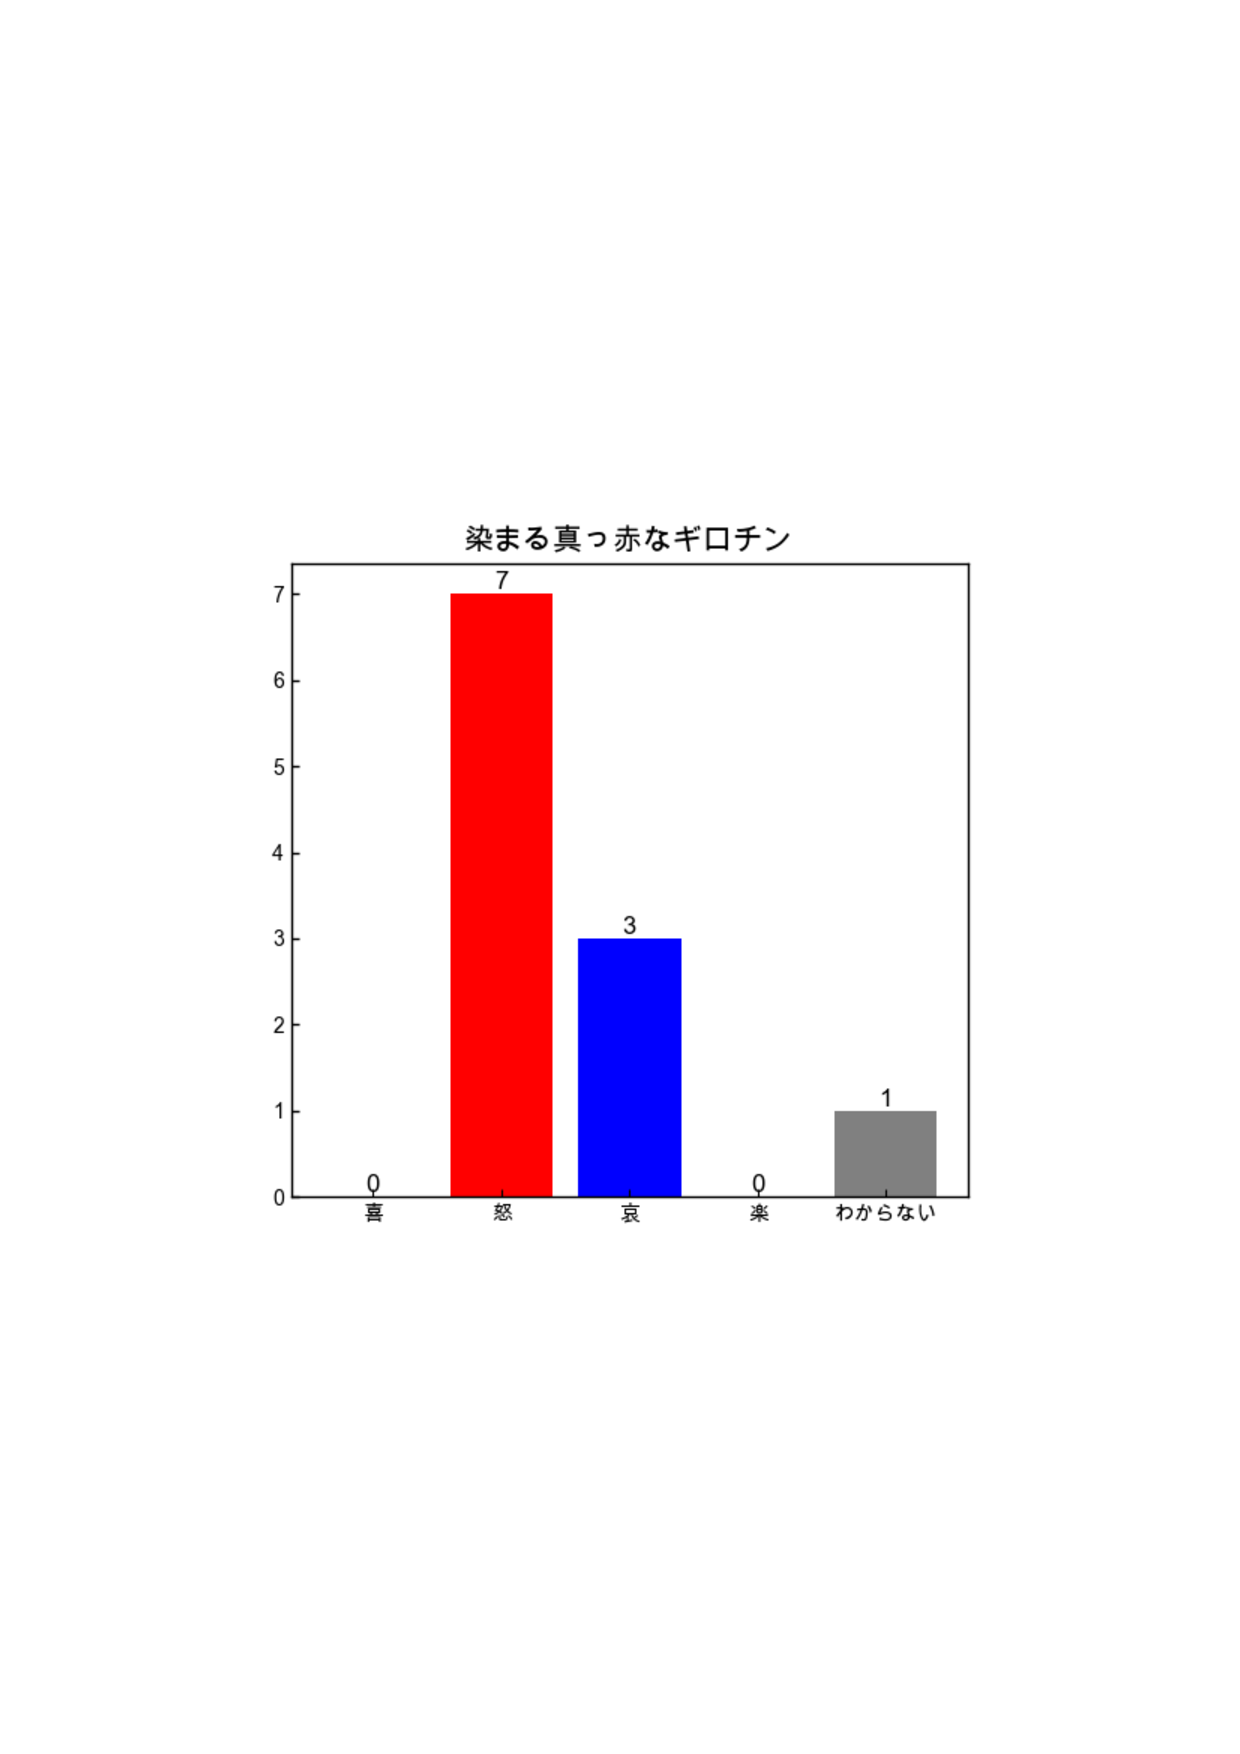
\includegraphics[width=14cm]{4311.pdf}
    \vspace{-1mm}
    \caption{フレーズ A-V+平面 第2グループ}
    \label{fig:mms}
    \vspace{5mm}
\end{figure}
第2グループから選出した「染まる真っ赤なギロチン」のフレーズから実験参加者0名が楽のクラスに感じたと回答した.
怒のクラスを感じたと回答した人数は5名,哀のクラスを感じたと回答した人数は3名,喜のクラスを感じた人はおらず,わからないと回答した人は1名であった.
実験参加者が推定した印象を感じていないことから推定結果は不当であるといえる.
\newpage
\begin{figure}[H]
    \centering
    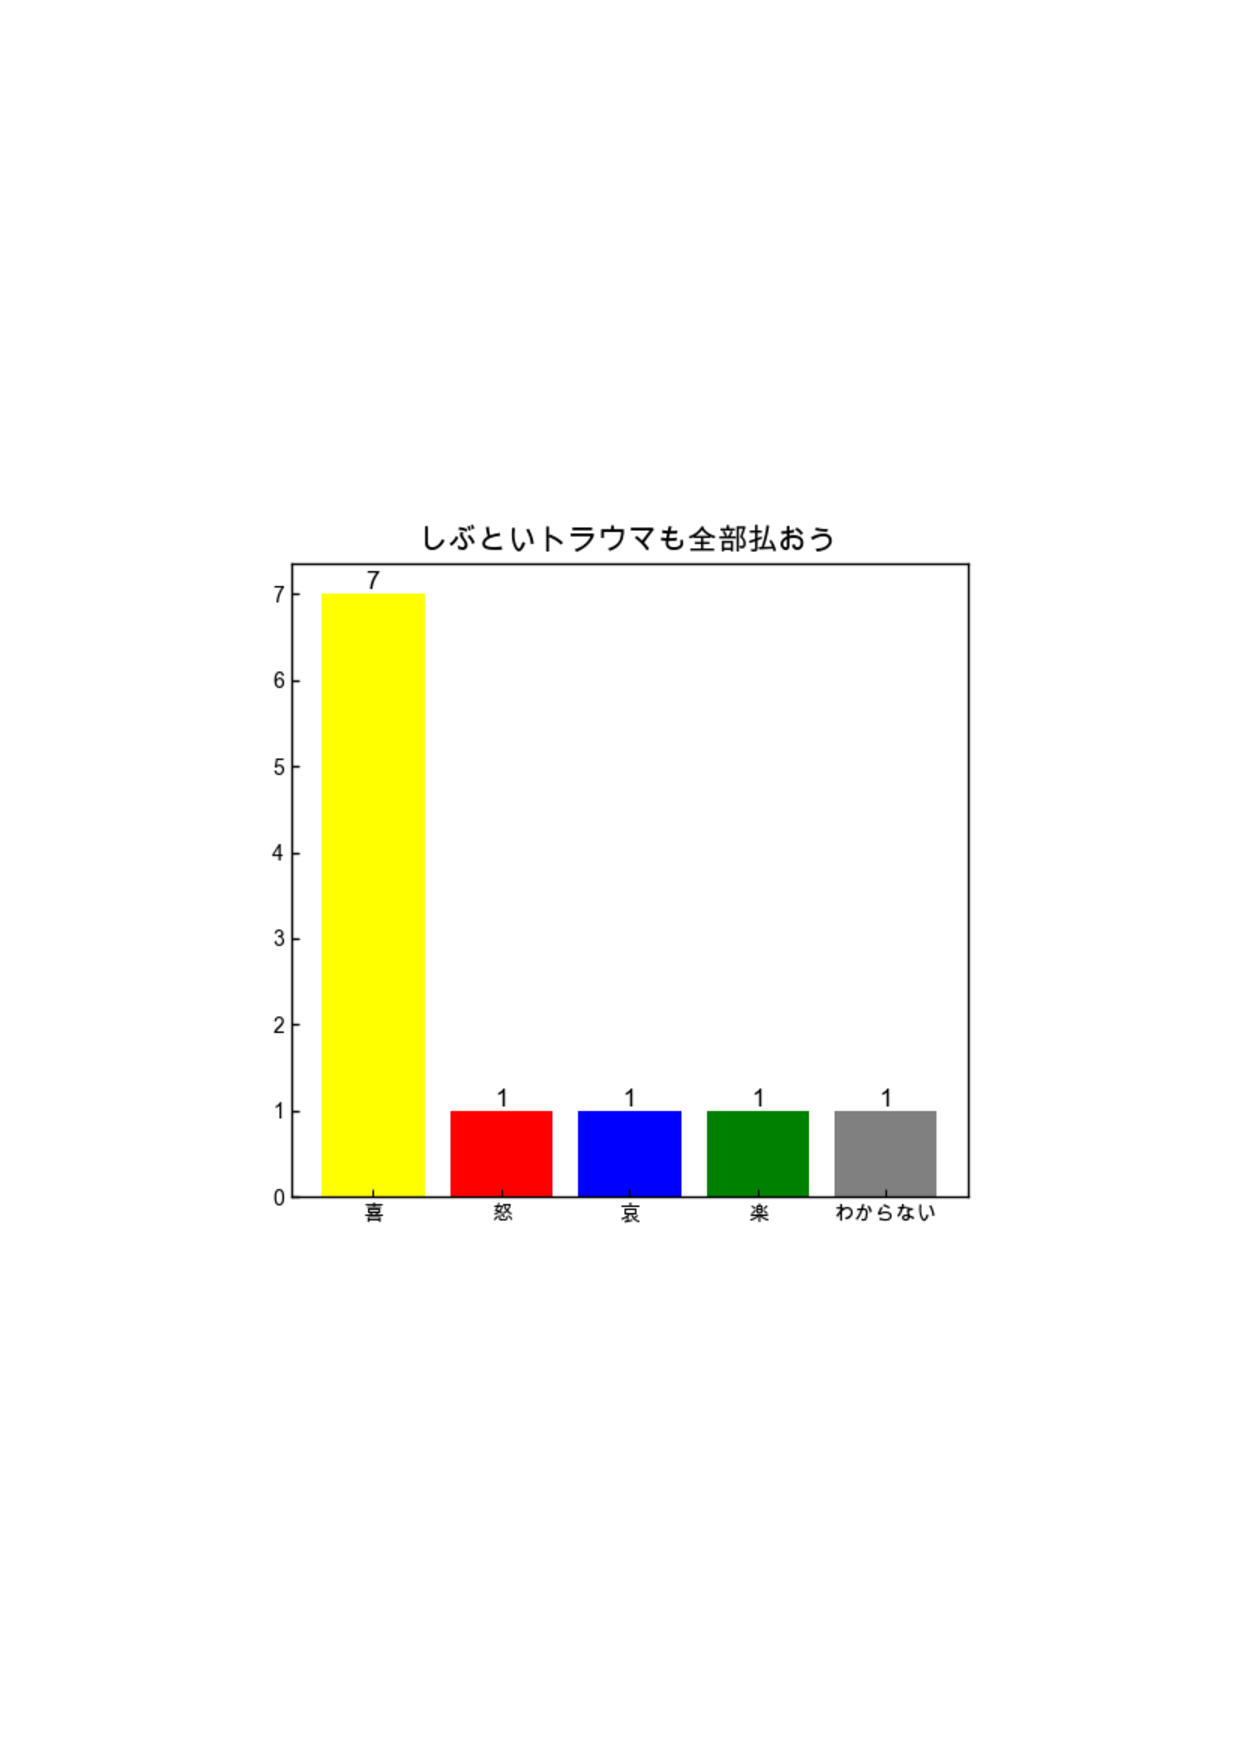
\includegraphics[width=14cm]{4312.pdf}
    \vspace{-1mm}
    \caption{フレーズ A-V+平面 第3グループ}
    \label{fig:mms}
    \vspace{5mm}
\end{figure}
第3グループから選出した「しぶといトラウマも全部払おう」のフレーズから実験参加者1名が楽のクラスに感じたと回答した.
喜のクラスを感じたと回答した人数は7名,怒と哀のクラスを感じた,またはわからないと回答した人はそれぞれ1名であった.
実験参加者が推定した印象を感じていないことから推定結果は不当であるといえる.
\newpage
